%%%%%%%%%%%%%%%%%%%%%%%%%%%%%%%%%%%%%%%%%%%%%%%%%%%%%%%%%%%%%%%%%%%%%%%%%%%%%%%%
%
% Template license:
% CC BY-NC-SA 3.0 (http://creativecommons.org/licenses/by-nc-sa/3.0/)
%
%%%%%%%%%%%%%%%%%%%%%%%%%%%%%%%%%%%%%%%%%%%%%%%%%%%%%%%%%%%%%%%%%%%%%%%%%%%%%%%%

%----------------------------------------------------------------------------------------
%	PACKAGES AND OTHER DOCUMENT CONFIGURATIONS
%----------------------------------------------------------------------------------------

\documentclass[
11pt, % The default document font size, options: 10pt, 11pt, 12pt
%oneside, % Two side (alternating margins) for binding by default, uncomment to switch to one side
%chapterinoneline,% Have the chapter title next to the number in one single line
spanish,
singlespacing, % Single line spacing, alternatives: onehalfspacing or doublespacing
%draft, % Uncomment to enable draft mode (no pictures, no links, overfull hboxes indicated)
%nolistspacing, % If the document is onehalfspacing or doublespacing, uncomment this to set spacing in lists to single
%liststotoc, % Uncomment to add the list of figures/tables/etc to the table of contents
%toctotoc, % Uncomment to add the main table of contents to the table of contents
parskip, % Uncomment to add space between paragraphs
%codirector, % Uncomment to add a codirector to the title page
headsepline, % Uncomment to get a line under the header
]{MastersDoctoralThesis} % The class file specifying the document structure



%----------------------------------------------------------------------------------------
%	INFORMACIÓN DE LA MEMORIA
%----------------------------------------------------------------------------------------

\thesistitle{Robot móvil de inspección y desinfección} % El títulos de la memoria, se usa en la carátula y se puede usar el cualquier lugar del documento con el comando \ttitle

% Nombre del posgrado, se usa en la carátula y se puede usar el cualquier lugar del documento con el comando \degreename
\posgrado{Carrera de Especialización en Sistemas Embebidos} 
%\posgrado{Carrera de Especialización en Internet de las Cosas} 
%\posgrado{Carrera de Especialización en Intelegencia Artificial}
%\posgrado{Maestría en Sistemas Embebidos} 
%\posgrado{Maestría en Internet de las cosas}

\author{Sergio Alberino} % Tu nombre, se usa en la carátula y se puede usar el cualquier lugar del documento con el comando \authorname

\director{Claudio Abel Verrastro (CNEA - UTN/FRBA)} % El nombre del director, se usa en la carátula y se puede usar el cualquier lugar del documento con el comando \dirname
\codirector{Nombre del codirector (pertenencia)} % El nombre del codirector si lo hubiera, se usa en la carátula y se puede usar el cualquier lugar del documento con el comando \codirname.  Para activar este campo se debe descomentar la opción "codirector" en el comando \documentclass, línea 23.

\juradoUNO{Eduardo Filomena (pertenencia)} % Nombre y pertenencia del un jurado se usa en la carátula y se puede usar el cualquier lugar del documento con el comando \jur1name
\juradoDOS{Juan Vicente Montilla Cabrera (pertenencia)} % Nombre y pertenencia del un jurado se usa en la carátula y se puede usar el cualquier lugar del documento con el comando \jur2name
\juradoTRES{Sergio Burgos (pertenencia)} % Nombre y pertenencia del un jurado se usa en la carátula y se puede usar el cualquier lugar del documento con el comando \jur3name

\ciudad{Ciudad Autónoma de Buenos Aires}
%\ciudad{ciudad de Mendoza}

\fechaINICIO{junio de 2020}
\fechaFINAL{junio de 2021}


\keywords{Sistemas embebidos, FIUBA} % Keywords for your thesis, print it elsewhere with \keywordnames


\begin{document}


\frontmatter % Use roman page numbering style (i, ii, iii, iv...) for the pre-content pages

\pagestyle{plain} % Default to the plain heading style until the thesis style is called for the body content


%----------------------------------------------------------------------------------------
%	RESUMEN - ABSTRACT 
%----------------------------------------------------------------------------------------

\begin{abstract}
\addchaptertocentry{\abstractname} % Add the abstract to the table of contents
%
%The Thesis Abstract is written here (and usually kept to just this page). The page is kept centered vertically so can expand into the blank space above the title too\ldots
\centering

En este trabajo se describe el desarrollo e implementación de un prototipo de robot móvil para tareas de desinfección por efecto de rayos ultravioletas. El dispositivo puede realizar un recorrido autónomo, evitando obstáculos en un ambiente cerrado, o puede controlarse en forma inalámbrica desde una tablet o celular, y será utilizado para desinfección en espacios públicos o en el hogar, y como plataforma para actividades de docencia e investigación en el Grupo de Inteligencia Artificial y Robótica de la Universidad Tecnológica Nacional Facultad Regional Buenos Aires
Para el desarrollo de este trabajo fueron fundamentales los conocimientos adquiridos de arquitectura de software, de programación de microcontroladores, protocolos de comunicaciones e interfaz con Bluetooth, como así también las metodologías de especificación de requerimientos de software.



\end{abstract}

%----------------------------------------------------------------------------------------
%	CONTENIDO DE LA MEMORIA  - AGRADECIMIENTOS
%----------------------------------------------------------------------------------------

\begin{acknowledgements}
%\addchaptertocentry{\acknowledgementname} % Descomentando esta línea se puede agregar los agradecimientos al índice
\vspace{1.5cm}

Esta sección es para agradecimientos personales y es totalmente \textbf{OPCIONAL}.  

\end{acknowledgements}

%----------------------------------------------------------------------------------------
%	LISTA DE CONTENIDOS/FIGURAS/TABLAS
%----------------------------------------------------------------------------------------

\tableofcontents % Prints the main table of contents

\listoffigures % Prints the list of figures

\listoftables % Prints the list of tables


%----------------------------------------------------------------------------------------
%	CONTENIDO DE LA MEMORIA  - DEDICATORIA
%----------------------------------------------------------------------------------------

\dedicatory{\textbf{Dedicado a... [OPCIONAL]}}  % escribir acá si se desea una dedicatoria

%----------------------------------------------------------------------------------------
%	CONTENIDO DE LA MEMORIA  - CAPÍTULOS
%----------------------------------------------------------------------------------------

\mainmatter % Begin numeric (1,2,3...) page numbering

\pagestyle{thesis} % Return the page headers back to the "thesis" style

% Incluir los capítulos como archivos separados desde la carpeta Chapters

% Chapter 1

\chapter{Introducción general} % Main chapter title

\label{Chapter1} % For referencing the chapter elsewhere, use \ref{Chapter1} 
\label{IntroGeneral}
En este capítulo se presentan las características de los robots de servicio, se  reseña el uso de luz ultravioleta como germicida y se exponen los objetivos que motivaron el presente trabajo y sus respectivo alcance.
%----------------------------------------------------------------------------------------

% Define some commands to keep the formatting separated from the content 
\newcommand{\keyword}[1]{\textbf{#1}}
\newcommand{\tabhead}[1]{\textbf{#1}}
\newcommand{\code}[1]{\texttt{#1}}
\newcommand{\file}[1]{\texttt{\bfseries#1}}
\newcommand{\option}[1]{\texttt{\itshape#1}}
\newcommand{\grados}{$^{\circ}$}

%----------------------------------------------------------------------------------------

%\section{Introducción}

%----------------------------------------------------------------------------------------
\section{Robots de servicio}

A lo largo del siglo XX la robótica pasó de ser una temática de la rama de la ciencia ficción, a cumplir un importante rol dentro de los complejos industriales. En los últimos años los robots han pasado a tener cada vez más tareas de “servicio” para ambientes  públicos y hogareños.
La robótica de servicios abarca un amplio campo de aplicaciones, la mayoría de las cuales tienen diferentes grados de automatización, desde la teleoperación completa hasta el funcionamiento autónomo, y constituye un campo de aplicación más diverso que el de la robótica industrial. En la  figura \ref{fig:robotsservicio} se pueden observar tres tipos de robots de servicios: una aspiradora hogareña, un cortador de césped y un limpiavidrios.

\begin{figure}[h]
	\centering
	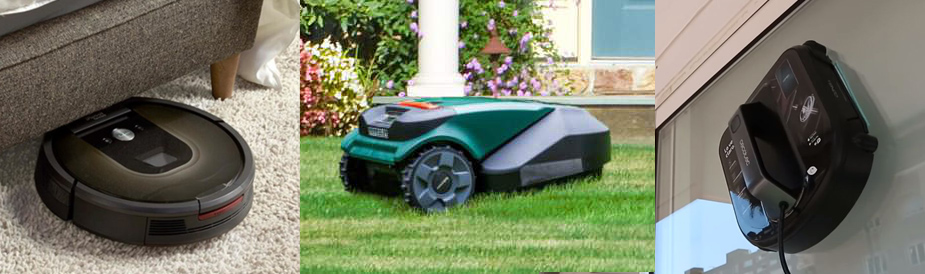
\includegraphics[width=\textwidth]{./Figures/robotsservicio.jpg}
	\caption{Robots de servicio\protect\footnotemark.}
	\label{fig:robotsservicio}
\end{figure}
\footnotetext{Imágenes tomadas de \url{https://www.domotizar.com/}}


A mediados de la década de 1990, la Comisión Económica de las Naciones Unidas para Europa (UNECE) \citep{UNECE} y la Federación Internacional de Robótica (IFR) \citep{IFR} adoptaron un sistema de clasificación de robots de servicio dividida por categorías y tipos de interacción, que se ha mantenido hasta la actualidad. En la  figura \ref{fig:robotsservicio} se puede observar los primeros ítems de clasificación para robots domésticos/personales de acuerdo a los tipos y áreas de aplicación.
\pagebreak


\begin{figure}[h]
	\centering
	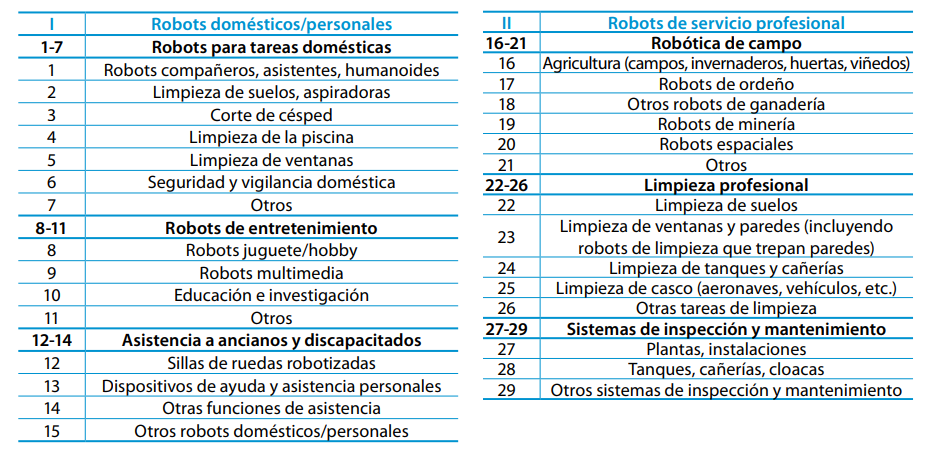
\includegraphics[width=\textwidth]{./Figures/clasificacion.png}
	\caption{Clasificación de robots de servicio\protect\footnotemark.}
	\label{fig:clasificacion}
\end{figure}
\footnotetext{Imagen tomada de \url{https://www.editores-srl.com.ar/sites/default/files/aa1_ifr_robots.pdf}}




\subsection{Robots móviles para inspección y limpieza}

Los robots móviles son dispositivos que poseen un sistema de locomoción capaz de navegar a través de un determinado ambiente de trabajo. Normalmente cuentan con cierto nivel de autonomía que les permite el desplazamiento sin colisiones por un recorrido específico. Sus aplicaciones son muchas y en general  están relacionadas con tareas monótonas o riesgosas para la salud humana.

Las plataformas móviles pueden realizar tareas de inspección y limpieza de manera autónoma o controlada remotamente por un operador. Son utilizadas en zonas de difícil acceso debido a limitaciones de espacio o razones de seguridad. Este tipo de robot suele contar con sensores de distinto tipo, para detectar los límites y obstáculos ante los que se presentan.
 
La proliferación de robots para limpieza se incrementó fuertemente a partir de la pandemia de Covid-19, con lo que se los puede encontrar hoy en día en espacios en los que antes no estaban presentes, tales como salas médicas,  hoteles y en el transporte público \citep{Cleaning}. 

Estos dispositivos “de interior” abarcan varios tipos. En la  figura \ref{fig:robotslimpieza} se puede observar un modelo de robot trapeador húmedo, una aspiradora robótica y un limpiavidrios automático, a modo de ejemplo.

\begin{figure}[h]
	\centering
	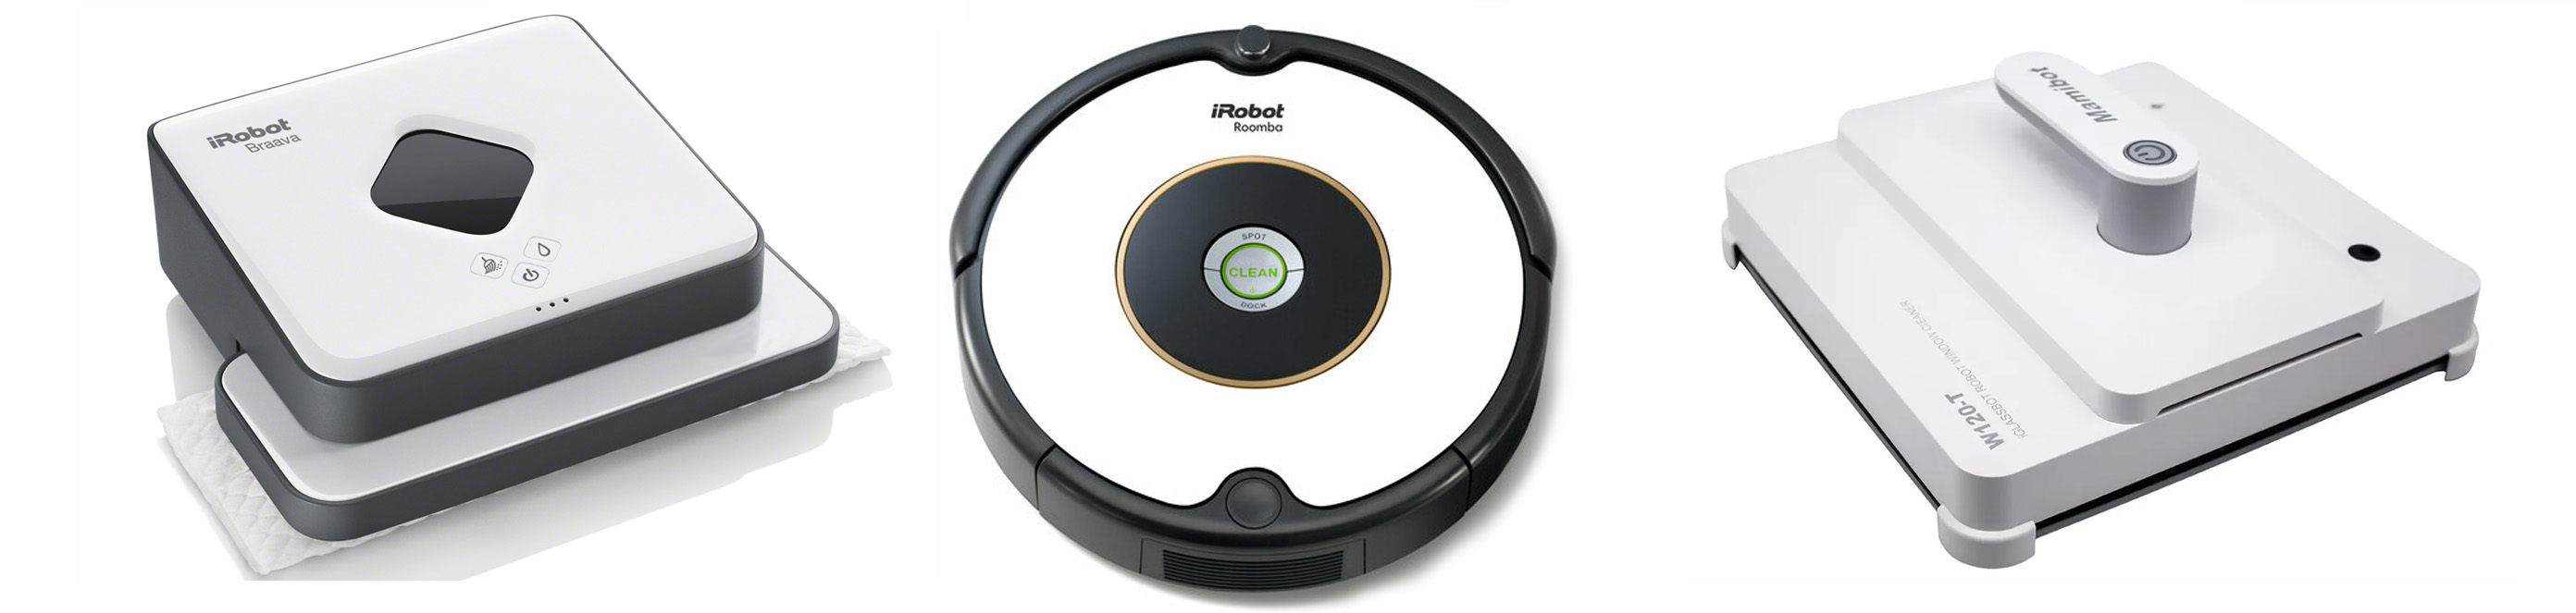
\includegraphics[width=\textwidth]{./Figures/robotslimpieza.jpg}
	\caption{Distintos tipos de robot de limpieza\protect\footnotemark.}
	\label{fig:robotslimpieza}
\end{figure}
\footnotetext{Imágenes tomadas de \url{https://www.domotizar.com/}}

Si bien todas las aspiradoras robots cumplen con la misma función básica de aspirar polvo y suciedad, las prestaciones de cada modelo y marca varían considerablemente junto con el precio de mercado. Los precios pueden oscilar entre los 200 y los 1200 dólares \citep{roomba}.
Los robots de mayor gama incorporan cepillos, trapeadores húmedos y/o luz ultravioleta germicida. Las versiones más van avanzadas  presentan mayor cantidad de sensores de proximidad a la vez que incorporan cámaras y rayos laser para medir distancias hasta los obstáculos.  
La navegación de los robots más simples es de tipo aleatoria, simplemente  sorteando los obstáculos con los que se encuentra y sin seguir una trayectoria ordenada. 
Robots más elaborados obtienen información del entorno usando cámaras o lasers, y construyendo un  mapa para planificar un recorrido que siga un orden específico. 


%----------------------------------------------------------------------------------------

\subsection{Robots de desinfección por luz ultravioleta}

Desde hace tiempo se utiliza luz ultravioleta para la desinfección de agua potable, y más recientemente ha sido incorporada como método germicida en conductos de ventilación. También se ha utilizado para la desinfección de instrumental e insumos en ambientes hospitalarios. En el  siguiente apartado se dará referencia acerca de la eficiencia de la luz ultravioleta, dentro de cierto rango de longitud de onda, para el control de bacterias y virus.

En los últimos dos años, con el aumento de precauciones debido a la pandemia mundial por el COVID-19, comenzaron a comercializarse robots móviles de luz ultravioleta germicida, para desinfectar quirófanos y salas de hospitales\citep{inventos}. 
Estos robots, poseen paneles con tubos ultravioleta para poder irradiar completamente una habitación o parte de la misma y son de alturas entre los 120 y los 180 cm para poder iluminar camas y mesas desde arriba y poder pasar por puertas y aberturas convencionales. En la figura \ref{fig:robotuv} se muestra un robot de estas características.

\begin{figure}[h]
	\centering
	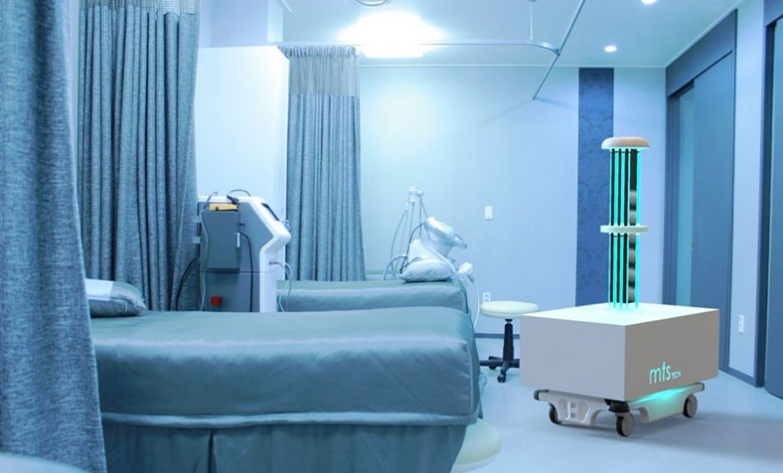
\includegraphics[width=12cm]{./Figures/robothospitalario.PNG}
	\caption{Robot desinfectante por luz ultravioleta en una sala de hospital\protect\footnotemark.}
	\label{fig:robotuv}
\end{figure}
\footnotetext{Imagen tomada de \url{https://www.infoplc.net/plus-plus/empresas/item/107726-mts-tech-robot-movil-ultravioleta-covid-19}}

La cobertura de los robots móviles de luz ultravioleta germicida suele ser mayor a los 180 grados, por lo que resulta importante no solo el recorrido realizado para abarcar todas las superficies, sino también evitar la presencia cercana de personas ya que la exposición de rayos ultravioleta puede ser perjudicial para la piel y la vista.  

Además de los hospitales, estos robots están siendo usados en otros espacios, como vagones del subterráneo, espacios comunes en hoteles, oficinas y áreas de control en aeropuertos \citep{masrobots}.

Otra aplicación que empieza a dársele a los robots UV-C es la desinfección fungicida en viñedos (en particular el oidio, que es un hongo que ataca todos los tejidos verdes del cultivo). Dispositivos robot recorren las plantaciones por la noche con paneles ultravioleta cuya luz daña el ADN del hongo, sin afectar a las plantas \citep{infowine}.

En 2020, la empresa argentina UV- Robotics lanzó el UVR-Robot \citep{UVR} que cuenta con tubos de luz UV-C germicida dispuestos en un arreglo de 360 grados para que la luz llegue hasta cualquier rincón y con una plataforma omnidireccional. El proceso toma  entre 5 y 15 minutos según la superficie, y se lo puede dirigir a control remoto. Esto le permite desinfectar autobuses, aviones y otros medios de transporte, salas de espera, centros de mayores, colegios, entidades bancarias, hoteles, ascensores o aseos. La iniciativa  tuvo el apoyo del Ministerio de Desarrollo Nacional y cuenta con validaciones y homologaciones de la Universidad Tecnológica Nacional. En la figura \ref{fig:uvrobot} se observa al UVR-Robot desinfectando un vagón de tren subterráneo. 

\begin{figure}[h]
	\centering
	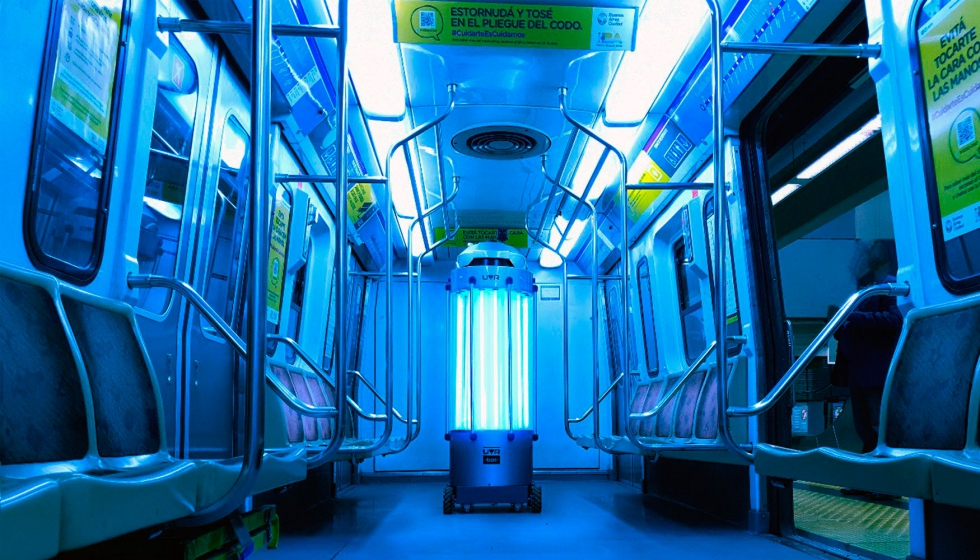
\includegraphics[width=12cm]{./Figures/uvrobot.jpeg}
	\caption{UVR-Robot de la agencia nacional UV- Robotics\protect\footnotemark.}
	\label{fig:uvrobot}
\end{figure}
\footnotetext{Imagen tomada de \url{https://www.interempresas.net/Tecnologia-aulas/Articulos/321010-UVR-bot-reto-acabar-cualquier-rastro-covid-19-20-minutos-luz-ultravioleta.html}}

A nivel hogareño, muchos robots de limpieza empiezan a incorporar la luz ultravioleta como medio de desinfección. En general, es una característica adicional que presentan las aspiradoras robóticas que además de barrido y trapeado húmedo agregan la esterilización de suelos con luz ultravioleta, resultando hoy en día una característica evaluada en las comparativas de los distintos productos  \citep{Bidcom}. En la figura \ref{fig:coradiruv} se observa la imagen de una aspiradora modelo Warptech ARobot 1000 UV con la funcionalidad de desinfección por UV-C por medio de LEDs ultravioletas en la parte inferior.


\begin{figure}[h]
	\centering
	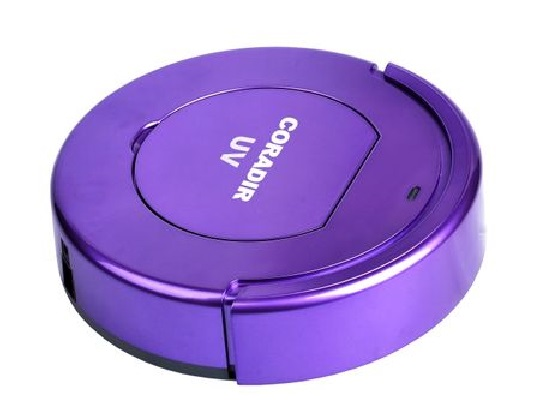
\includegraphics[width=5cm]{./Figures/coradiruv.jpg}
	\caption{Imagen de la aspiradora Warptech ARobot 1000 UV\protect\footnotemark.}
	\label{fig:coradiruv}
\end{figure}
\footnotetext{Imagen tomada de \url{https://www.coradir.com.ar/producto/productos_categoria/aspiradoras-roboticas}}


También se han comenzado a comercializar  robots móviles de las dimensiones de una aspiradora robot, pero con el único fin de esterilizar gérmenes y virus usando la emisión de luz UV-C de baja intensidad (sin aspiradora o trapeador), para empresas y comercios en general. La propuesta que presentan es la dejar al robot funcionando por la noche en los espacios que se desean desinfectar. Un ejemplo de esta aplicación es el robot germicida móvil por UV-C y ozono  Conga Apolo \citep{conga} de la empresa española Cecotec. Su precio se encuentra alrededor de los 1000 euros.


%----------------------------------------------------------------------------------------
\section{Desinfección usando luz ultravioleta}

El espectro ultravioleta (UV) abarca la banda de radiación electromagnética entre los 400 y 100 nm, presentando una longitud de onda menor que la de la luz visible y mayor que la de los rayos X.  Se divide en las siguientes categorías principales:

\begin{itemize}
	\item los rayos UV-A (400 – 315 nm), que son los más cercanos al espectro visible.
	\item los rayos UV-B (315 – 280 nm), que son absorbidos en gran parte por diferentes elementos a medida que atraviesan el cielo.
	\item los rayos UV-C (280 – 200 nm), que son absorbidos totalmente por la capa de ozono.
\end{itemize}

En la  figura \ref{fig:espectro} se observa la  clasificación de luz según longitud de onda en  espectro de radiación electromagnética.

\begin{figure}[h]
	\centering
	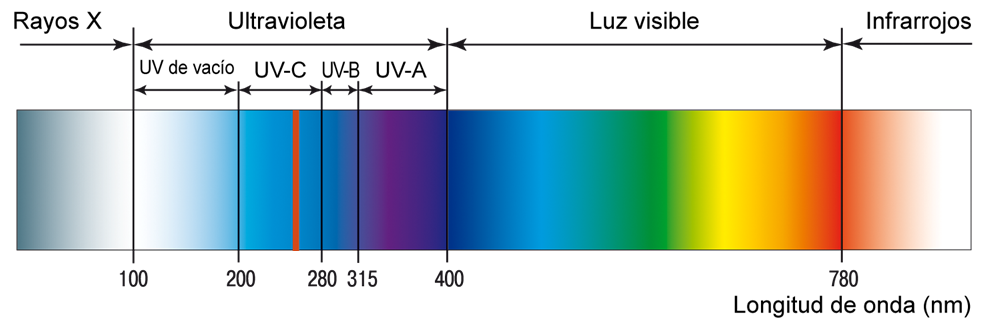
\includegraphics[width=14cm]{./Figures/espectro.PNG}
	\caption{Clasificación de luz según longitud de onda\protect\footnotemark.}
	\label{fig:espectro}
\end{figure}
\footnotetext{Imagen tomada de \url{https://www.lit-uv.com/es/technology/}}

%\pagebreak

La utilización de luz ultravioleta UV-C como germicida ha demostrado efectividad para la esterilización  las bacterias, gérmenes, virus, algas y esporas. 

Los virus tienen un tamaño inferior a un micrómetro (µm, una millonésima parte de un metro) y las bacterias son típicamente de 0,5 a 5 µm. Técnicamente es incorrecto decir que los rayos  UV-C matan a los virus, siendo que no se trata de organismos vivientes. Sin embargo, el comité de foto-biología de la \emph{ Illuminating Engineering Society} (IES) informa que los fotones UV-C interactúan con el ARN y las moléculas de ADN en un virus o bacteria de modo que se evita su reproducción y por lo tanto su efecto infeccioso. Una célula que no puede reproducirse se considera muerta; ya que no puede multiplicarse dentro del anfitrión. A este proceso se lo denomina “desactivación”   \citep{IES}. En la figura \ref{fig:adn} se representa el efecto de la luz UV-C en el ADN de bacterias, gérmenes, virus, algas y esporas. 
 

\begin{figure}[h]
	\centering
	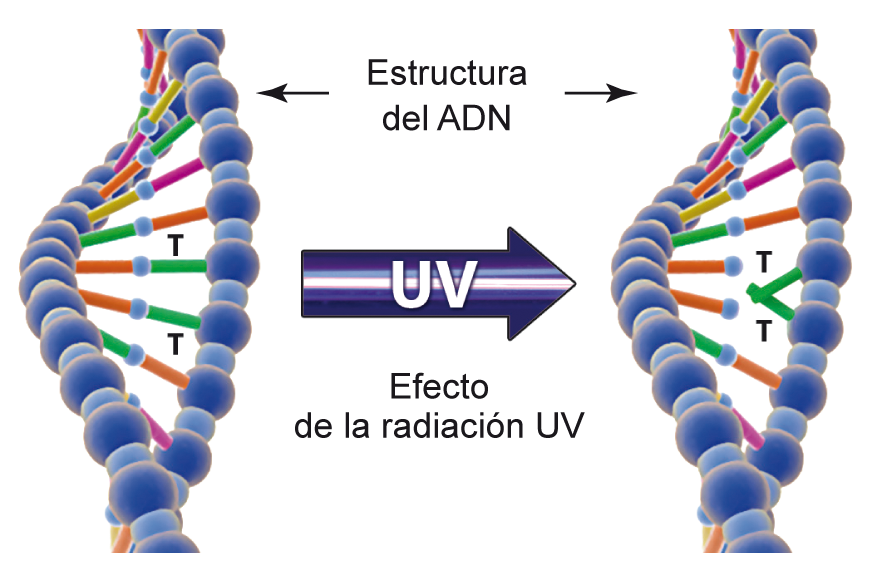
\includegraphics[width=9cm]{./Figures/adn.png}
	\caption{Efecto de la UV-C sobre el ADN de microorganismos\protect\footnotemark.}
	\label{fig:adn}
\end{figure}
\footnotetext{Imagen tomada de \url{https://www.lit-uv.com/es/technology/}}

La \emph{International Ultraviolet Association}  (IUVA) afirma que los resultados de pruebas en laboratorio de desinfección utilizando UV-C entre los 200 y 280 nm demuestran especial utilidad para reducir la transmisión de los virus causantes del COVID-19:  SARS-CoV-1 y MERS-CoV \citep{IUA}. En la práctica, el efecto depende de factores tales como  el tiempo de exposición y obstrucción que puedan tener los rayos para alcanzar plenamente los pliegues u ondulaciones que pudiera tener la superficie a desinfectar. 

En un informe sobre utilización de la radiación ultravioleta para desinfección \citep{CSIC}, el Consejo Superior de Investigaciones Científicas de España, concluye que el uso de radiación UV-C es muy adecuado para la desinfección de microorganismos y de virus, y propone su uso en combinación con métodos tradicionales para la desinfección en  zonas de alta contaminación.

La cantidad de inactivación de patógenos en superficies es directamente proporcional a la dosis de radiación UV-C, definida como el producto de la intensidad (W/m2) por la duración de la exposición. La dosis de luz UV necesaria varía en función del patógeno que se quiera desinfectar y de las condiciones ambientales\citep{CIE}.

Una de las ventajas de este método de desinfección radica en que una vez terminada el ambiente puede volver a ser utilizado inmediatamente, ya que no existe radiación persistente. La desinfección  por UV-C resulta además menos contaminante para el medio ambiente, al no exponer al ser humano a los riesgos derivados del uso de productos químicos. La desinfección germicida por ultravioleta es especialmente recomendada cuando debe realizarse sobre materiales que podrían verse afectados o dañados ante la limpieza continua con productos a base de químicos líquidos, como ser dispositivos electrónicos o materiales susceptibles a la  oxidación \citep{interior}. 
%En la figura \ref{fig:gabineteuv} se muestra un gabinete utilizado para la desinfección ultravioleta de toallas, pinzas, cortauñas, limpieza de cepillos de dientes, teléfono móvil, etc.
%%\vspace{12mm}
%
%\begin{figure}[h]
%	\centering
%	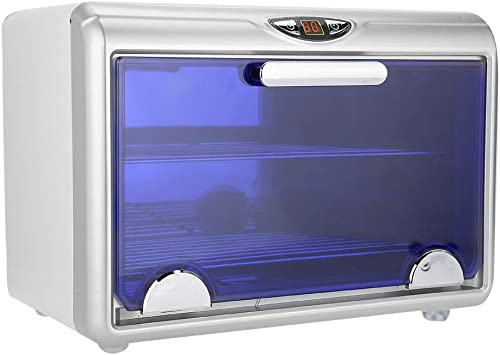
\includegraphics[width=7cm]{./Figures/gabineteuv.jpg}
%	\caption{Ejemplo de gabinete de desinfección ultravioleta.}
%	\label{fig:gabineteuv}
%\end{figure}

Existen también dispositivos portátiles de esterilización con LEDs ultravioleta en la longitud de onda entre los 200 y 280 nm para desinfectar celulares, teclados, llaves, juguetes para bebés y otros objetos pequeños. Se trata de luz de baja potencia (menor a los 15 mW) pero fuertemente enfocada sobre la superficie a esterilizar, desde una distancia muy corta (menor a los 3 cm), con lo que aprovechan al máximo la energía radiada. El tiempo de  aplicación de la luz UV sobre la superficie oscila entre los 30 y 60 segundos, según la potencia del dispositivo. En la figura \ref{fig:esterilizador} se observa una imagen de un modelo de esterilizador portátil por UV-C. Muchos de estos dispositivos justifican su eficiencia con un estudio realizado en 2020 por el Guangdong Detection Center of Microbiology \citep{Guangdong}.   


\begin{figure}[h]
	\centering
	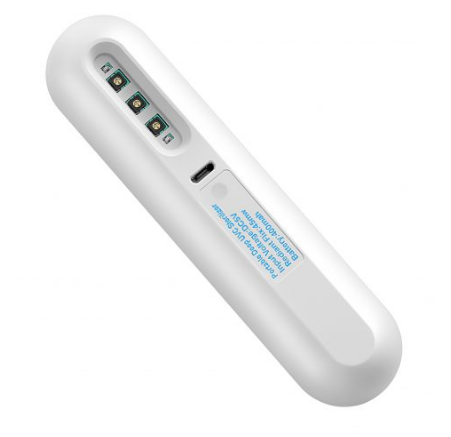
\includegraphics[width=4cm]{./Figures/esterilizador.PNG}
	\caption{Ejemplo de esterilizador portátil por UVC\protect\footnotemark.}
	\label{fig:esterilizador}
\end{figure}
\footnotetext{Imagen tomada de \url{https://procid.cl/producto/luz-led-germicida-portatil-uv-c-blanco/}}


La desinfección por rayos UV-C es también útil en el caso de superficies de difícil acceso por su ubicación o cuando la zona presenta formas y estructuras que no permiten la higienización por contacto con paños o rociadores. 

Por otra parte, la irradiación con luz UV-C presenta una serie de limitaciones. El patógeno que desea esterilizarse debe ser  expuesto directamente a la radiación para que sea eliminado. Si bien la Organización Mundial de la Salud (OMS) recomienda el uso de rayos UV-C para desinfección, también alerta sobre los riesgos de  exposición en seres humanos y animales, cuya piel puede verse irritada, a la vez que puede producir daños a la vista \citep{MYTH}. En este sentido promueven la limpieza periódica de manos con jabón o con alcohol, y dejan la esterilización con UV-C para  instrumental y objetos de uso diario.



%----------------------------------------------------------------------------------------

\section{Motivación}

Existen cada vez más robots de servicio orientados a tareas específicas de ayuda para la industria y para el hogar. 
Debido al avance de la pandemia por COVID-19, en 2020 proliferaron los robots  para desinfección utilizando emisión de luz ultravioleta de tipo germicida. Se trata de dispositivos de grandes dimensiones (con alturas entre uno y dos metros) ya que buscan cubrir superficies amplias como las de salas de hospitales, almacenes, espacios de transportes públicos, etc. Al mismo, tiempo se ha visto que muchos robots de limpieza hogareña empiezan a incorporar la desinfección por UV-C como parte de sus prestaciones. 
En un informe sobre utilización de la radiación ultravioleta para desinfección \citep{CSIC} elaborado por el Consejo Superior de Investigaciones Científicas de España, se propone como algo necesario el diseño de robots móviles que recorran superficies horizontales de forma autónoma irradiando luz UV-C para la desinfección de ambientes cerrados.

En función de estas cuestiones, y con el fin de elaborar un trabajo acorde al nivel de los temas planteados en la especialización en sistemas embebidos, es que surge la idea de construir una plataforma móvil de dimensiones similares a las de una aspiradora robot comercial, que pudiera utilizarse para desinfección por rayos UV-C en espacios cerrados y sobre superficies planas, donde puedan existir obstáculos (patas de mesas, sillas, etc.) que dificulten la limpieza por otros medios (trapeadores, cepillos). El dispositivo puede ser usado para desinfección sin residuos químicos en espacios públicos (salas de atención médica, instituciones educativas) y en el hogar. También podría resultar conveniente para esterilizar superficies que no pueden ser limpiadas con productos líquidos, como es el caso de losetas de caucho o productos similares, como las utilizadas en jardines de infantes o gimnasios. En la figura \ref{fig:ruvot} se observa una representación del robot para tareas de desinfección con UV-C.


\begin{figure}[h]
	\centering
	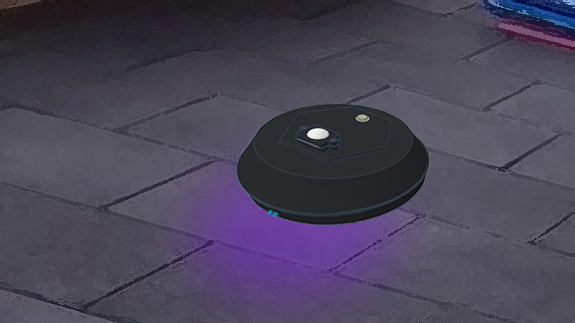
\includegraphics[width=10cm]{./Figures/rUVot14.png}
	\caption{Repressentación del robot para tareas de desinfección por UV-C.}
	\label{fig:ruvot}
\end{figure}


Si bien existen plataformas robot con fines educativos y de experimentación, la mayoría son de fabricación extranjera y de costos elevados para ser afrontados por instituciones educativas. La construcción de prototipos robóticos a nivel nacional constituye en ese sentido un buen aporte para ampliar el parque de plataformas de experimentación y desarrollo de nuevas aplicaciones.

Se espera que el hardware resultante del presente trabajo pueda ser aprovechado en el Grupo de Inteligencia Artificial y Robótica de la UTN - Facultad Regional Buenos Aires, para la evaluación de algoritmos de Inteligencia Artificial. La placa EDU-CIAA cuenta con capacidad suficiente para el procesamiento de algoritmos reactivos para la planificación de recorridos con obstáculos (compatibles con trabajos realizados), en los que intervenga aprendizaje por refuerzo o comportamientos “aprendidos” con una red neuronal. 

%----------------------------------------------------------------------------------------

\section{Objetivos y alcances}


El propósito de este trabajo es el desarrollo de un prototipo de robot móvil para ser utilizado en tareas de desinfección por efecto de rayos ultravioletas germicidas.
El dispositivo posee un modo autónomo en el que realiza un recorrido aleatorio dentro de una habitación evitando obstáculos detectados por los sensores, y un modo de teleoperación en el que puede controlarse a distancia (de unos metros) desde una aplicación en un celular o tablet a través de Bluetooth.

El prototipo se diseñó para que una superficie plana sea irradiada con un dispositivo emisor de rayos ultravioletas de tipo C en forma teleoperada o haciendo un recorrido autónomo aleatorio, aceptando las propiedades germicidas en las emisiones de este rango de longitud de onda (entre los 200 y 280 nm). 

En todos los casos, el uso de este robot móvil constituye un aporte a la desinfección de ambientes cerrados, que no implica que deba dejarse de lado los métodos tradicionales de prevención y limpieza. 


Se utilizan sensores infrarrojos y de contacto para evitar los obstáculos que puedan aparecer en el camino del robot. La información sensada se maneja en forma de valores booleanos, para simplificar el procesamiento, tanto en uso de memoria como en velocidad. 

El comportamiento general, en el modo autónomo, puede ser reconfigurado a través de una tabla disponible en una librería del programa, y generada por una aplicación en PC. Esto permite cambiar el comportamiento reactivo del robot, sin modificar la rutina principal de procesamiento, basada en máquina de estados.


La plataforma posee una placa de procesamiento central (EDU-CIAA) que recibe datos y una placa de control para el accionamiento de motores y/o dispositivos adicionales (como puede ser el encendido de LEDs UV-C germicidas). En la figura \ref{fig:blocks} se puede apreciar un diagrama con los principales bloques del dispositivo.


\begin{figure}[h]
	\centering
	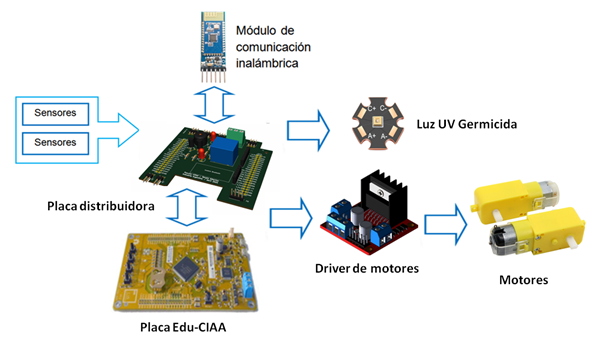
\includegraphics[width=\textwidth]{./Figures/blocks.png}
	\caption{Repressentación del robot para tareas de desinfección por UV-C.}
	\label{fig:blocks}
\end{figure}

Se construyó además un prototipo mecánico para contener las distintas partes de hardware electrónico, como así también pode observar el comportamiento de sensores y motores en su conjunto.
Si bien el prototipo contempla el recorrido sobre el piso, irradiando luz ultravioleta hacia abajo, no hay ningún impedimento para que los se sensores se monten de forma que el robot pueda recorrer una superficie plana elevada (una mesa de trabajo, por ejemplo) sin caerse, o que el emisor de luz se encuentre en la parte lateral o superior (dado que es controlado en forma independiente).

No se plantean pruebas funcionales que demuestren que se han esterilizado microorganismos y de virus al utilizar el dispositivo, siendo que eso implicaría ensayos y estudios que exceden el equipamiento disponible y las aéreas de estudio de la especialización en sistemas embebidos.

El robot se alimenta con baterias recargables. No se  monitorea   ni se realiza la carga de las baterías. No se incluye cargador.



%----------------------------------------------------------------------------------------
\chapter{Introducción específica} % Main chapter title

\label{Chapter2}

%----------------------------------------------------------------------------------------
%	SECTION 1
%----------------------------------------------------------------------------------------
En este capítulo se presentan las distintas tecnologías y metodologías disponibles para la implementación del prototipo de robot móvil. Se describen los dispositivos más significativos que permitieron alcanzar los requerimientos planteados.

\section{Diseño del prototipo}

El prototipo se diseñó para que una superficie plana sea irradiada con un dispositivo emisor de rayos ultravioletas de tipo C en forma teleoperada o haciendo un recorrido autónomo aleatorio.

Se utilizaron sensores infrarrojos y de contacto para evitar los obstáculos que puedan aparecer en el camino del robot. La información sensada se maneja en forma de valores booleanos, para simplificar el procesamiento, tanto en uso de memoria como en velocidad. 

La plataforma posee una placa de procesamiento central (EDU-CIAA) que recibe datos y una placa de control para el accionamiento de motores y/o dispositivos adicionales (como puede ser el encendido de LEDs UV-C germicidas). En la figura \ref{fig:blocks} se puede apreciar un diagrama con los principales bloques del dispositivo.


\begin{figure}[h]
	\centering
	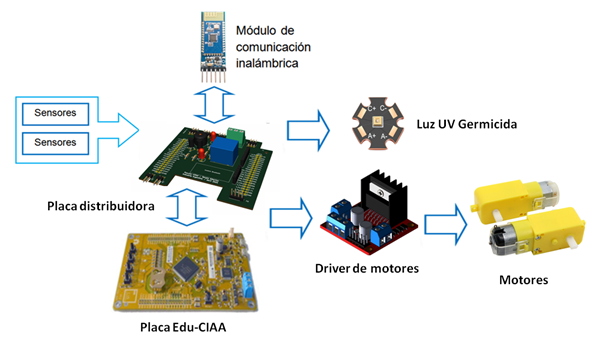
\includegraphics[width=\textwidth]{./Figures/blocks.png}
	\caption{Repressentación del robot para tareas de desinfección por UV-C.}
	\label{fig:blocks}
\end{figure}

El comportamiento general, en el modo autónomo, puede ser reconfigurado a través de una tabla disponible en una librería del programa, y generada por una aplicación en PC. Esto permite cambiar el comportamiento reactivo del robot, sin modificar la rutina principal de procesamiento, basada en máquina de estados.

Se construyó una estructura mecánica para contener las distintas partes de hardware electrónico, y poder ensayar el comportamiento de sensores y motores en su conjunto.

Si bien el prototipo robot contempla el recorrido sobre el piso, irradiando luz ultravioleta hacia abajo, no hay ningún impedimento para que los sensores se monten de forma que el robot pueda recorrer una superficie plana elevada (una mesa de trabajo, por ejemplo) sin caerse, o que el emisor de luz se encuentre en la parte lateral o superior (dado que es controlado en forma independiente).

No se plantean pruebas funcionales que demuestren que se han esterilizado microorganismos y virus al utilizar el dispositivo, dado que esto implicaría ensayos y estudios que exceden el equipamiento disponible y las aéreas de estudio de la especialización en sistemas embebidos.

El robot se alimenta con baterias recargables. No se  monitorea   ni se realiza la carga de las baterías y no se incluye cargador.
%----------------------------------------------------------------------------------------

\section{Módulos y dispositivos de hardware}
En esta sección se describen los módulos y dispositivos de hardware utilizados en el prototipo del robot desarrollado.

%----------------------------------------------------------------------------------------
\subsection{Placa de microprocesamiento}

Se decidió utilizar como hardware principal la placa de desarrollo EDU-CIAA-NXP \citep{EDUCIAA} para aprovechar la experiencia existente en la comunidad del posgrado.

En la figura \ref{fig:EDUCIAANXP} se observa una imagen de la EDU-CIAA-NXP, una versión de bajo costo de la CIAA-NXP, pensada para la enseñanza universitaria, terciaria y secundaria. 

\begin{figure}[htpb]
	\centering
	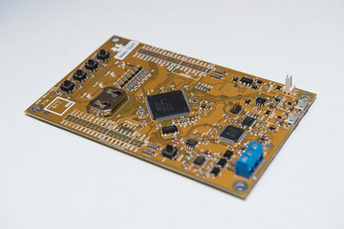
\includegraphics[width=\textwidth]{./Figures/EDUCIAANXP.jpg}
	\caption{Placa de desarrollo EDUCIAA-NXP\protect\footnotemark.}
	\label{fig:EDUCIAANXP}
\end{figure}
\footnotetext{Imagen tomada de \url{http://www.proyecto-ciaa.com.ar}}

\pagebreak

En la figura \ref{fig:Bloques} puede verse un diagrama en bloques general de la placa. 

\begin{figure}[htpb]
	\centering
	\includegraphics[width=9cm]{./Figures/Bloques.jpg}
	\caption{Diagrama en bloques de la EDUCIAA-NXP\protect\footnotemark.}
	\label{fig:Bloques}
\end{figure}
\footnotetext{Imagen tomada de \url{http://www.proyecto-ciaa.com.ar}}

El  microcontrolador utilizado por la EDU-CIAA es el LPC4337 (dual core ARM Cortex-M4F y Cortex-M0). Los recursos más significativos que se utilizaron de la placa fueron: 


\begin{itemize}
	\item GPIO (General Purpose Input/Output, Entrada/Salida de Propósito General)
	\item PWM (Pulse Width Modulation, modulación por ancho de pulso).
	\item UART (Universal Asynchronous Receiver-Transmitter, Transmisor-Receptor Asíncrono Universal).
	\item Temporizadores.
\end{itemize}

Para el accionamiento de los motores se utilizó modulación por ancho de pulsos (PWM, por su sigla en inglés). La placa EDU-CIAA posee un solo modulo PWM con 11 salidas asociadas. Todas las salidas PWM comparten la misma frecuencia, aunque puede asignarse un valor de ciclo de actividad en forma independiente.

%\begin{itemize}
%	\item PWM0:  GPIO\_2.
%	\item PWM1:  GPIO\_8.
%	\item PWM2:  T\_FIL1.
%	\item PWM3:  T\_FIL2.
%	\item PWM4:  T\_FIL3.
%	\item PWM5:  T\_COL0.
%	\item PWM6:  T\_COL1.
%	\item PWM7:  T\_COL2.
%	\item PWM8:  LCD\_1.
%	\item PWM9:  LCD\_2.		
%	\item PWM10: LCD\_3.				
%\end{itemize}
%
%Se utilizaron las líneas de T\_FIL3: PWM4 y T\_COL1: PWM6 para el control de los motores.


%----------------------------------------------------------------------------------------
\subsection{Motores}

El robot es impulsado por dos motores de corriente continua con reducción mecánica.

Para la selección de los motores se tuvieron en cuenta las características del prototipo a desarrollar. 
Las opciones típicas para este tipo de robot son los motores de corriente continua, los motores paso a paso y los servomotores \citep{servo}. 


En la tabla \ref{tab:comparacion} se listan ventajas y desventajas de estos tipos de motor.

 
\begin{table}[htpb]
\centering
\caption[comparacion]{Comparación de características según tipo de motor.}


\begin{tabular}{llll}
\hline
            & Motor de CC                                                                              & Motor paso a paso                                                                                                                                 & Servomotor                                                                                                                       \\ \hline
Ventajas    & \begin{tabular}[c]{@{}l@{}}Alta velocidad\\ y torque.\\ Fácil de controlar.\end{tabular} & \begin{tabular}[c]{@{}l@{}}Control de \\ posición sin \\ realimentación.\\ Precisión en \\ el control de \\ posición y \\ velocidad.\end{tabular} & \begin{tabular}[c]{@{}l@{}}Alta precisión \\ en control de \\ posición y \\ velocidad. \\ Circuito \\ realimentado.\end{tabular} \\ \hline
Desventajas & \begin{tabular}[c]{@{}l@{}}Requiere \\ reducción \\ mecánica.\end{tabular}               & \begin{tabular}[c]{@{}l@{}}Requiere \\ controlador.\\ Baja potencia.\end{tabular}                                                                 & \begin{tabular}[c]{@{}l@{}}Limitación\\ del recorrido. \\ Costoso.\end{tabular}                                                  \\ \hline
\end{tabular}
\label{tab:comparacion}
\end{table}

Los motores de corriente continua pueden alcanzar altas velocidades y un alto torque. Son fáciles de controlar, pero requieren de reducciones mecánicas cuando la velocidad de operación es baja.
Los motores paso a paso presentan precisión en sus movimientos sin requerir de realimentación,  pero exigen mayor electrónica para su control. Son muy efectivos para realizar desplazamientos cortos y precisos. Los servomotores  tienen un desplazamiento angular limitado y presentan gran precisión en movimientos cortos. Su principal  desventaja radica en el costo relativamente alto.

Se seleccionaron motores de corriente continua con caja reductora debido a que ofrecen las prestaciones suficientes para este tipo de robot, sin requerir de controladores (de hardware o software) adicionales \citep{motorcc}. 
En la figura \ref{fig:motorreductor} se puede ver una imagen del motor utilizado.

\begin{figure}[h]
	\centering
	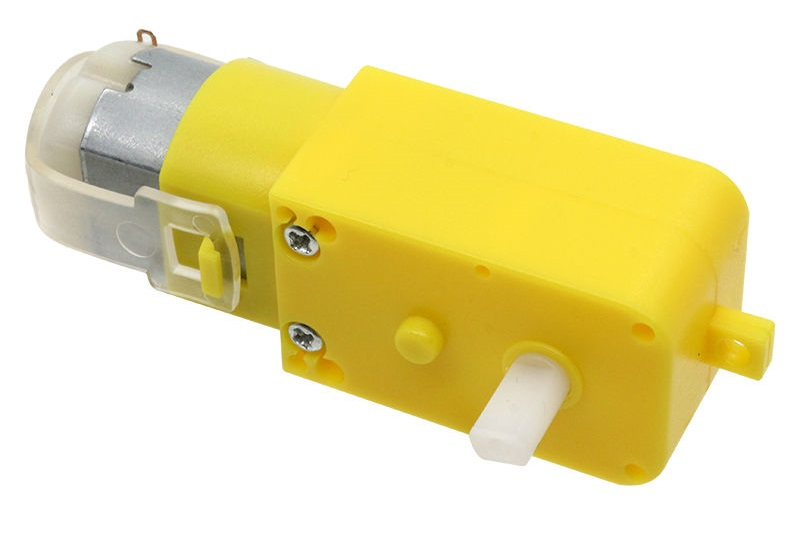
\includegraphics[width=7cm]{./Figures/Motorreductor.jpg}
	\caption{Imagen del motor utilizado\protect\footnotemark.}
	\label{fig:motorreductor}
\end{figure}
\footnotetext{Imagen tomada de \url{https://robots-argentina.com.ar/}}

Los motores elegidos cuentan con una caja de reducción (48:1) acoplada al eje del motor eléctrico, para lograr la disminución de velocidad, y un eje lateral que permite reducir espacio al utilizarlos en una configuración diferencial. La tensión nominal de trabajo va de los  3 a 6 V. Este modelo de motorreductor es ampliamente difundido en el mercado de componentes para robótica didáctica, por lo que es de fácil adquisición y bajo costo. 

En la tabla \ref{tab:caracteristicas} se referencian las principales características de los motores, según su tensión nominal de alimentación. 

\begin{table}[htpb]
\centering
\caption[características]{Características de los motores.}
\begin{tabular}{lccc}
                    & 3V DC       & 5V DC       & 6V DC      \\ \hline
Reducción           & \multicolumn{3}{c}{48:1}               \\
Velocidad sin carga & 125 RPM     & 200 RPM     & 230 RPM    \\
Velocidad con carga & 95 RPM      & 152 RPM     & 175 RPM    \\
Torque              & 0,8 kg.cm   & 1 kg.cm     & 1,1 kg.cm  \\
Corriente           & 110-130 mA  & 120-140 mA  & 130-150 mA \\
Dimensiones         & \multicolumn{3}{c}{70mm x 22mm x 18mm} \\
Peso                & \multicolumn{3}{c}{50g}                \\
Ruido               & \multicolumn{3}{c}{\textless{}65dB} 		\\  \hline
\end{tabular}
\label{tab:caracteristicas}
\end{table}


%En la figura \ref{fig:planomoto} se pueden observar las dimensiones del motor utilizado.
%
%%
%\pagebreak
%
%\begin{figure}[h]
%	\centering
%	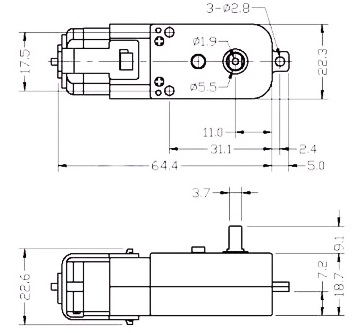
\includegraphics[width=9cm]{./Figures/planomoto.jpg}
%	\caption{Dimensiones del motor utilizado\protect\footnotemark.}
%	\label{fig:planomoto}
%\end{figure}
%\footnotetext{Imagen tomada de \url{https://robots-argentina.com.ar/}}





\subsection{Driver de motores}
Para el accionamiento de los motores se decidió utilizar un módulo basado en el circuito integrado L298N \citep{L298}. Este módulo tiene una configuración de doble puente H que permite  controlar dos motores de corriente continua de manera simultánea e independiente. 
El módulo ofrece conectores de entrada y salida para el puente integrado, un regulador LM78M05 interno que suministra 5V para la lógica de control, y los  los diodos de protección de contracorriente en las salidas \citep{Driver}.

En la figura \ref{fig:Driver} se puede observar una imagen de la placa y sus conectores. Sus características principales son:

\begin{itemize}
	\item Tensión mínima: 5 V.
	\item Tensión máxima: 35 V.
	\item Corriente máxima: 2 A.
	\item Tensión de nivel lógico: 5 V.
	\item Potencia máxima 25 W.
	\item Medidas: 43 x 43 x 24 mm.
\end{itemize}
%\pagebreak

\begin{figure}[h]
	\centering
	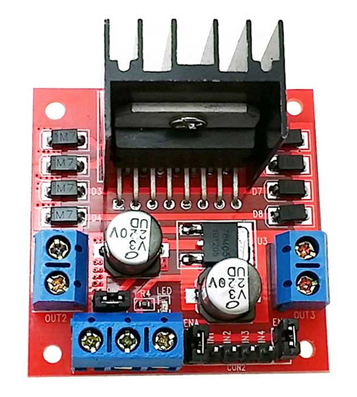
\includegraphics[width=6cm]{./Figures/L298N.png}
	\caption{Driver de motores\protect\footnotemark.}
	\label{fig:Driver}
\end{figure}
\footnotetext{Imagen tomada de \url{http://robots-argentina.com.ar}}


La placa tiene la opción de habilitar o no el regulador LM7805 integrado para alimentar la parte lógica. En la figura \ref{fig:Esquema} se observa el diagrama esquemático del módulo.


\begin{figure}[h]
	\centering
	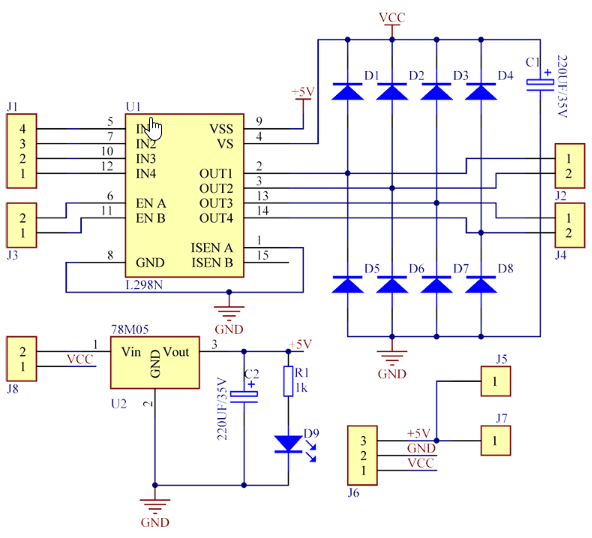
\includegraphics[width=11cm]{./Figures/Modulo.png}
	\caption{Diagrama esquemático del módulo\protect\footnotemark.}
	\label{fig:Esquema}
\end{figure}
\footnotetext{Imagen tomada de \url{http://robots-argentina.com.ar}}


%----------------------------------------------------------------------------------------

\subsection{Módulo sensor de infrarrojos}

Se utilizaron dos módulos sensores de proximidad por infrarrojos IR FC-51 \citep{IR} para la detección de obstáculos por parte del robot. Estos módulos están compuestos por  un emisor de luz infrarroja (IR)  y un receptor que detecta su reflejo en  las superficies contra las que se enfrenta, de modo que presentan una señal en  presencia de cualquier obstáculo en su parte frontal. 

El sensor presenta una respuesta estable incluso con luz ambiente o en completa oscuridad. En la figura \ref{fig:moduloIR} se observa una imagen del sensor de infrarrojos.

\begin{figure}[h]
	\centering
	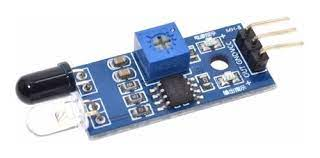
\includegraphics[width=8cm]{./Figures/moduloIR.jpg}
	\caption{Módulo sensor de infrarrojos \protect\footnotemark.}
	\label{fig:moduloIR}
\end{figure}
\footnotetext{Imagen tomada de \url{http://robots-argentina.com.ar}}

Las características del módulo son:
\begin{itemize}
	\item Ángulo de cobertura: 35°.
	\item Tensión de funcionamiento: 3 V – 6 V.
	\item Rango de detección: 2 cm – 30 cm (ajustable con el potenciómetro).
	\item Tamaño: 4,5 cm x 1,4 cm x 0,7 cm. 
	\item Discriminación: la salida toma nivel lógico bajo cuando se detecta un obstáculo (reflexión).
\end{itemize}

El circuito electrónico del módulo se basa en un amplificador operacional integrados LM339 utilizado como comparador entre la señal obtenida del receptor infrarrojo y un nivel de tensión determinado por un potenciómetro, lo cual permite ajustar el rango de distancia de la detección de obstáculo. En la figura \ref{fig:IRschem} se muestra el circuito esquemático del sensor de infrarrojos

\begin{figure}[h]
	\centering
	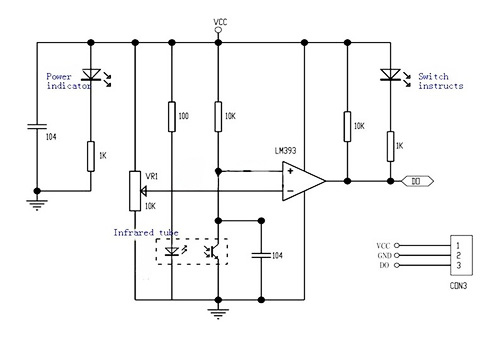
\includegraphics[width=14cm]{./Figures/IRschem.jpg}
	\caption{Diagrama esquemático del módulo sensor de infrarrojos\protect\footnotemark.}
	\label{fig:IRschem}
\end{figure}
\footnotetext{Imagen tomada de \url{http://robots-argentina.com.ar}}
%\pagebreak




%----------------------------------------------------------------------------------------
\subsection{Módulo detector pasivo de infrarrojos}

Se utilizó un módulo detector pasivo de infrarrojos (PIR) para poder sensar movimientos alrededor del robot cuando está encendido el módulo UV-C y desactivarlo para evitar la irradiación sobre personas o animales que se acerquen al robot. 
Los detectores PIR captan la variación de las radiaciones infrarrojas del medio ambiente que los rodea y de esa manera reaccionan ante fuentes de energía tales como el calor del cuerpo humano o de animales. Es llamado pasivo debido a que no emite radiaciones, sino que las recibe. Su funcionamiento se basa en un sensor piroeléctrico que es un componente electrónico diseñado para detectar cambios en la radiación infrarroja recibida. 

Se utilizó un módulo PIR HC-SR501 \citep{PIR} que cuenta con dos potenciómetros para regular la sensibilidad y el tiempo de duración del pulso. Las principales características son:

\begin{itemize}
	\item Tensión de operación: 4,5 V - 20 V.
	\item Corriente en reposo: <50 uA.
	\item Rango de detección: 3 a 7 metros (ajustable).
	\item Tiempo de retardo: 5 - 200 Seg (puede ser ajustado).
	\item Angulo de detección: <100º (cono).
	\item Tamaño: 3,2 cm x 2,4 cm x 1,8 cm.
\end{itemize}

En la figura \ref{fig:pir} se puede ver una imagen del módulo PIR HC-SR501 utilizado.

\begin{figure}[h]
	\centering
	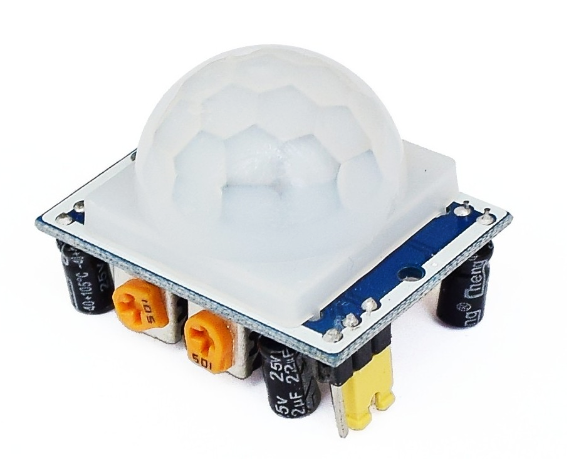
\includegraphics[width=8cm]{./Figures/pir.PNG}
	\caption{Módulo PIR HC-SR501\protect\footnotemark.}
	\label{fig:pir}
\end{figure}
\footnotetext{Imagen tomada de \url{https://naylampmechatronics.com/}}


%----------------------------------------------------------------------------------------
\subsection{Buzzer o transductor electroacústico}

Se utilizó un buzzer o transductor electroacústico para la señalización sonora sobre el estado de operación del robot. El transductor produce un tono audible, generado por un diafragma piezoeléctrico. 
El buzzer seleccionado es de tipo Activo, es decir que posee un oscilador incorporado al dispositivo. 
Sus características técnicas son:

\begin{itemize}
	\item Tensión de operación: 3,3 V ~ 5 V.
	\item Corriente de operación: <25 mA.
	\item Salida de sonido min a 10 cm: 85 dB.
	\item Frecuencia: 3,1 kHz. 	
	\item Diámetro: 12 mm.
	\item Altura: 7,5 mm.
	\item Longitud: 7,5 mm.	
\end{itemize}


En la figura \ref{fig:buzzer2} se observa imagen del transductor electroacústico utilizado.

\begin{figure}[h]
	\centering
	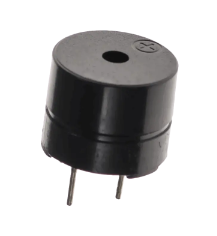
\includegraphics[width=3cm]{./Figures/buzzer2.PNG}
	\caption{Imagen del buzzer seleccionado\protect\footnotemark.}
	\label{fig:buzzer2}
\end{figure}
\footnotetext{Imagen tomada de \url{https://sumador.com/products/buzzer-activo-5v-12x9-5mm}}
%%

%----------------------------------------------------------------------------------------
\subsection{LED ultravioleta }

El robot cuenta con un relé para la activación del módulo UV-C. De esta manera el dispositivo emisor de luz ultravioleta puede tener alimentación independiente y hasta intercambiarse por otro de distintas prestaciones.
Para el desarrollo del prototipo se optó por un emisor LED de alta potencia, alimentado con la misma batería del robot, siendo que   son más compactos y resistentes a los golpes que las lámparas ultravioleta halógenas y emiten menos radiación de calor, por lo que pueden montarse más fácilmente sin tener que contar con disipadores adicionales. 
Los LEDs UV-C presentan un ángulo de apertura que oscila alrededor de los 120 grados con lo que es más fácil dirigir toda la potencia de radiación UV a una superficie específica.
Se utilizó un LED de alta potencia, germicida, tipo SMD3535, para el módulo de desinfección. Sus características técnicas son las siguientes:

\begin{itemize}
	\item Tipo de LED:		SMD3535.
	\item Color:		Ultravioleta UVC .
	\item Potencia:		1 W.
	\item Corriente		120 mA.	
	\item Tensión de Entrada:	5 a 8 VDC.
	\item Flujo Radiante:	7 - 12 mW.
	\item Longitud de Onda:	280 nm.
	\item Apertura del Haz:	140 grados.	
	\item Vida útil:	30000 horas.	
	\item Diámetro:		6,5 mm.	
	\item Largo:		15,5 mm.	
	\item Ancho:		8 mm.		
	\item Alto:			5,2 mm.		
	\item Peso: 		120 g.		
\end{itemize}


En la figura \ref{fig:leduvc} se observa imagen del LED UVC Germicida.

\begin{figure}[h]
	\centering
	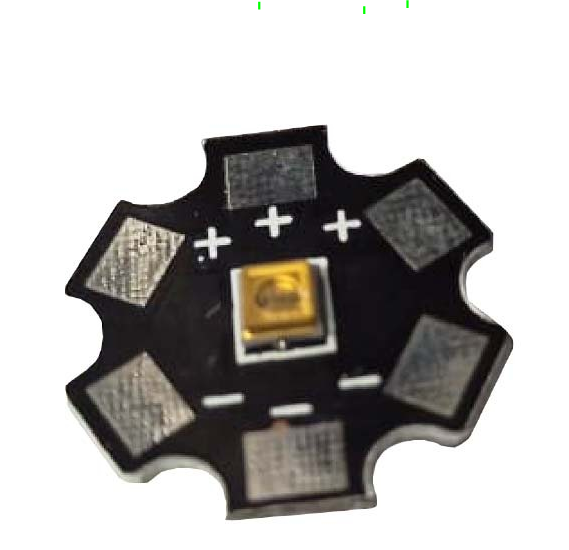
\includegraphics[width=4cm]{./Figures/leduvc.PNG}
	\caption{imagen del LED UVC Germicida seleccionado\protect\footnotemark.}
	\label{fig:leduvc}
\end{figure}
\footnotetext{Imagen tomada de \url{https://www.dled.com.ar}}
%%

%----------------------------------------------------------------------------------------
\subsection{Módulo de comunicaciones Bluetooth}

%Siendo que el prototipo robot se diseñó para su uso en ambientes interiores, la distancia del enlace no requiere un valor mayor al de algunos metros. Además la tasa de transferencia de datos no es alta, por lo que el ancho de banda no constituye un parámetro limitante. 

Se utilizó el módulo Bluetooth HC-05 para la comunicación con el robot \citep{HC05}. El mismo ya había sido utilizado en  prácticas de la asignatura "protocolos de comunicación en sistemas embebidos”.
El módulo permite realizar un enlace digital con un alcance de 10 m aproximadamente y no requiere antena externa ya que se encuentra integrada en el PCB. La velocidad máxima de transmisión asincrónica es de 2 Mbps y soporta modo master y modo slave.

En la figura \ref{fig:moduloHC05} se observa el módulo HC-05.


\begin{figure}[h]
	\centering
	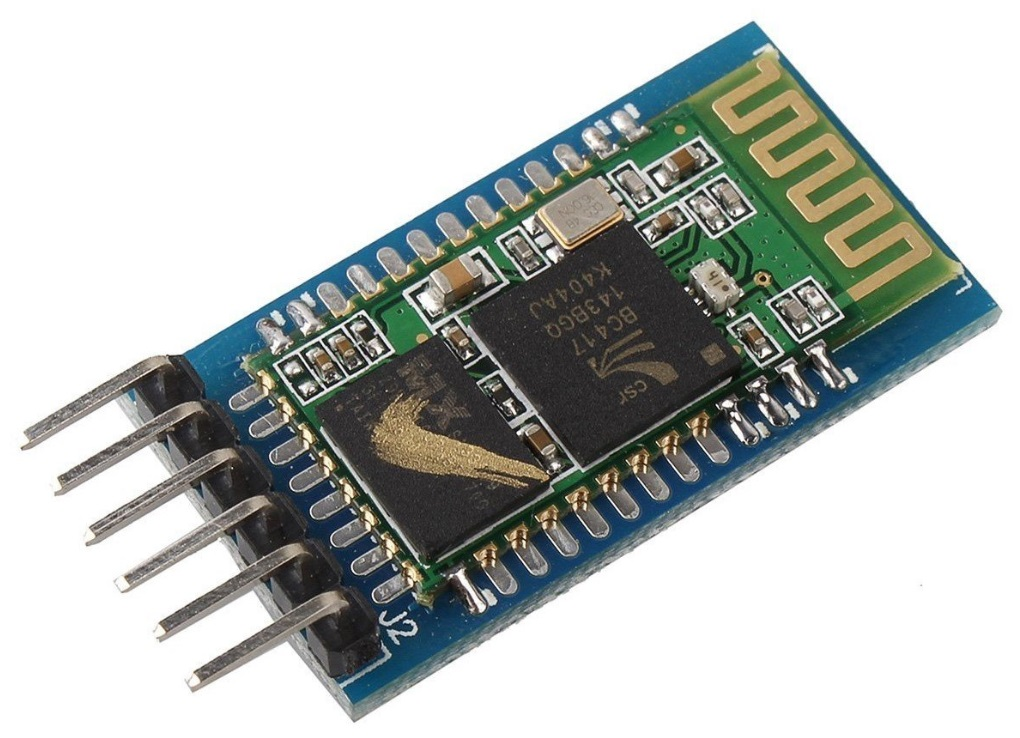
\includegraphics[width=6cm]{./Figures/HC05.jpeg}
	\caption{Módulo Bluetooth HC-05\protect\footnotemark.}
	\label{fig:moduloHC05}
\end{figure}
\footnotetext{Imagen tomada de \url{https://www.todomicro.com.ar/arduino/222-modulo-bluetooth-hc05}}


Las características del módulo son:
\begin{itemize}
	\item Tensión de operación: 3,6 V - 6 V DC.
	\item Consumo corriente: 50 mA.
	\item Bluetooth: V2.0+EDR.
	\item Frecuencia: banda ISM 2,4 GHz.
	\item Modulación: GFSK (Gaussian Frequency Shift Keying).
	\item Potencia de transmisión: 4 dBm, Class 2.
	\item Sensibilidad: -84 dBm a 0.1\% BER.
	\item Alcance 10 m.
	\item Tamaño: 3,7 cm x 1,6 cm.
\end{itemize}

El módulo HC-05 está configurado de fábrica como dispositivo esclavo (slave), pero se puede cambiar para que trabaje como maestro (master). También es posible modificar el nombre, código de vinculación, velocidad y otros parámetros mediante comandos AT \citep{HC05}. 

%\pagebreak


\subsection{Baterías}

En función del consumo y la intensión de no dedicar mayor espacio a las celdas de alimentación, se emplearon dos baterías de Ion-litio tipo 18650. La capacidad de estas baterías varía de un modelo a otro pero suelen estar comprendidas entre los 2100 y los 4000 mAh, y  permiten ser recargadas con una media de entre 600 a 1000 veces sin que se estropeen ni pierdan efectividad \citep{18650}. Su tensión nominal es de 3,7V, e incluso puede alcanzar los 4,2V en vacío.

Las baterías van conectadas en serie para lograr una tensión de 7,4 V, acorde a la alimentación de los motores, y con un margen superior necesario para el correcto funcionamiento del regulador de tensión de 5 V del módulo de accionamiento de motores. 
Las baterías se insertaron en un portapilas comercial. En la figura \ref{fig:portapila} se muestra las dos baterías 18650 ya instaladas en su portapila.


\begin{figure}[h]
	\centering
	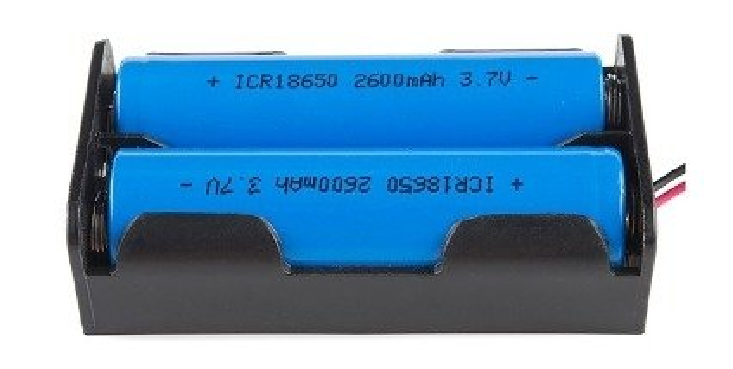
\includegraphics[width=10cm]{./Figures/portapilas.PNG}
	\caption{Baterías 18650 en su portapila .}
	\label{fig:portapila}
\end{figure}



%\section{Módulos de software}
%%En esta sección se describen los módulos de software utilizados.
%
%Se utilizaron módulos de software de la biblioteca sAPI \citep{sapi} del firmware de la EDU-CIAA versión 3 para acceder de manera simple a los diferentes periféricos.

\section{Entorno gráfico para el desarrollo de la aplicación móvil}

Para el desarrollo de la aplicación móvil se utilizó MIT App Inventor. Se trata de un entorno gráfico de programación desarrollado por Google Lab y administrado por el Instituto Tecnológico de Massachusett (MIT)\citep{MIT}, que utiliza un lenguaje visual basado en bloques el cual permite en forma sencilla programar aplicaciones totalmente funcionales para dispositivos que utilicen el sistema operativo Android \citep{android}.
La herramienta es de distribución gratuita y aunque las aplicaciones desarrolladas  en este entorno no alcanzan una gran complejidad, es posible cubrir con ellas un gran número de necesidades básicas en un dispositivo móvil.

El entorno cuenta con un módulo de diseño denominado App Inventor Designer con el que se desarrolla el contenido y la apariencia de la aplicación. En la figura \ref{fig:mitappdes} se observa la pantalla de diseño.

\begin{figure}[h]
	\centering
	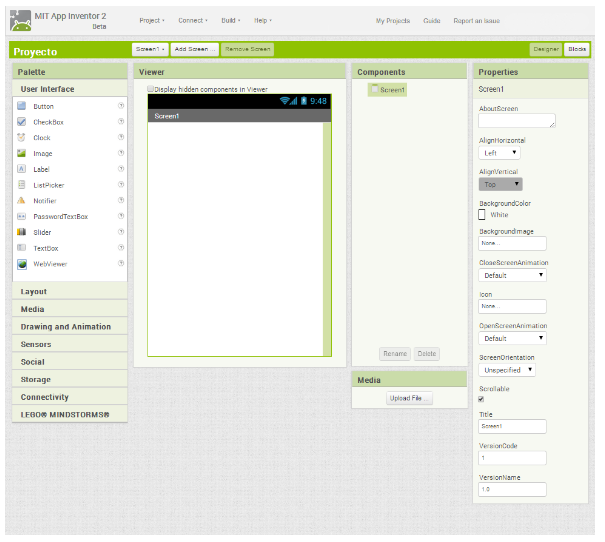
\includegraphics[width=12cm]{./Figures/appinventordesigner.PNG}
	\caption{Pantalla del módulo App Inventor Designer\protect\footnotemark..}
	\label{fig:mitappdes}
\end{figure}
\footnotetext{Imagen tomada de \url{https://diocesanos.es/blogs/equipotic/2015/05/16/mit-app-inventor-programando-aplicaciones-para-android/}}


Para la programación de la aplicación MIT App Inventor cuenta con un módulo editor de bloques denominado App Inventor Blocks Editor, que permite la programación en forma visual del comportamiento de los distintos  componentes de la aplicación, al ensamblar los bloques como piezas de un esquema. En la figura \ref{fig:mitappblock} se observa cómo se conforma el programa usando el editor de bloques.


\begin{figure}[h]
	\centering
	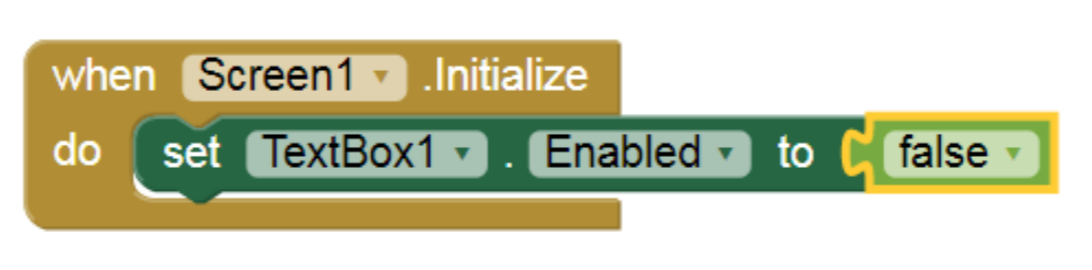
\includegraphics[width=8cm]{./Figures/mitblock.PNG}
	\caption{Ejemplo de programación en bloques usando App Inventor Blocks Editor.\protect\footnotemark..}
	\label{fig:mitappblock}
\end{figure}
\footnotetext{Imagen tomada de \url{https://docs.google.com/presentation/d/1jKjbLS9AFnHildJjZ8o4Jd7ou_ejwAmtdI0GGi0Jg48}}


Como aspecto positivo del uso de MIT App Inventor cabe resaltar que se trata de un software gratuito y de fácil configuración, al que se puede acceder desde cualquier computadora sin necesidad de instalarlo
Las limitaciones principales del uso de MIT App Inventor radican en que solo permite desarrollos para la plataforma Android, y que no se puede acceder a la interfaz de desarrollo (IDE) sin conexión a internet.

%\pagebreak

%%----------------------------------------------------------------------------------------
%%	SECTION 2
%%-----------------------------------------------------------------
%\section{Requerimientos}
%
%En esta sección se enumeran los requerimientos planteados en la planificación inicial del proyecto.  Los  requerimientos se han dividido en funcionales y no funcionales.
%
%\label{sec:requerimientos}
%
%\begin{enumerate}
%\item Requerimientos funcionales
%	\begin{enumerate}
%	\item Capacidad de locomoción.  El robot debe ser capaz de desplazarse por medio de ruedas motorizadas, a través de superficies planas.
%	\item Capacidad de percepción. El robot debe ser capaz de detectar y obtener información del medio. 
%	\item Capacidad de comunicación inalámbrica. El robot sebe ser capaz de establecer una comunicación  por medio de un módulo Bluetooth, con una aplicación android en un celular o tablet.
%	\item El robot deberá funcionar con alimentación a batería recargable.
%	\item El proyecto debe ser extensible a una posible herramienta de enseñanza e investigación.
%
%	\end{enumerate}
%\item Requerimientos no funcionales
%	\begin{enumerate}
%	\item El robot no debe emitir luz UV-C cuando detecte movimiento a su alrededor, para no producir daños a la salud de personas o animales con los que interactue.
%	\item El diseño del robot debe respetar regulaciones en cuanto a radiación en el espectro ultravioleta.
%	\item Se utilizarán componentes electrónicos disponibles comercialmente en Argentina.
%	\end{enumerate}
%\end{enumerate}
%
%%\section{Planificación}
%%
%%El trabajo se organizó para ser terminado en el mes de junio de 2021 con una dedicación aproximada de 600 horas en total, mientras se realizaba la cursada de la especialización en sistemas embebidos.
%%
%%\subsection{Diagrama de Gantt}
%%Con el fin de organizar y dar seguimiento a las actividades requeridas y poder identificar los desvíos en los tiempos de ejecución programados, se cuantificaron los tiempos de las diversas tareas mediante el diagrama de Gantt, que se observa en las figuras \ref{fig:gantt1} y \ref{fig:gantt2}.
%%
%%
%%\begin{figure}[htpb]
%%\centering 
%%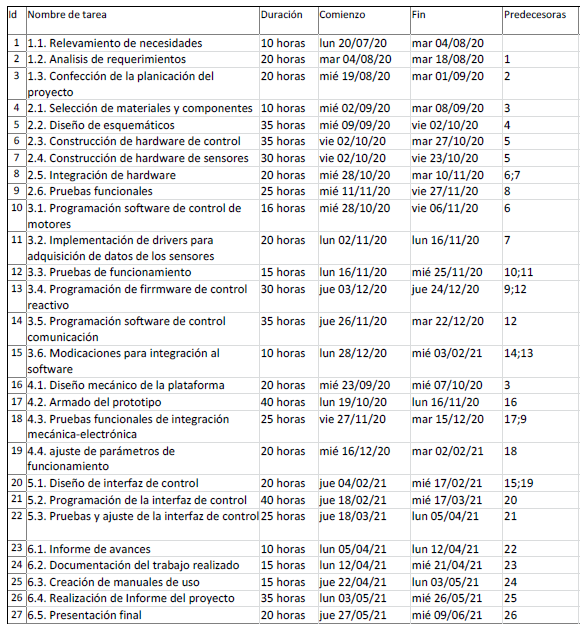
\includegraphics[width=\textwidth]{./Figures/gantttabla.PNG}
%%\caption{Tabla de tareas de Gantt.}
%%\label{fig:gantt1}
%%\end{figure}
%%
%%\begin{figure}[htpb]
%%\centering 
%%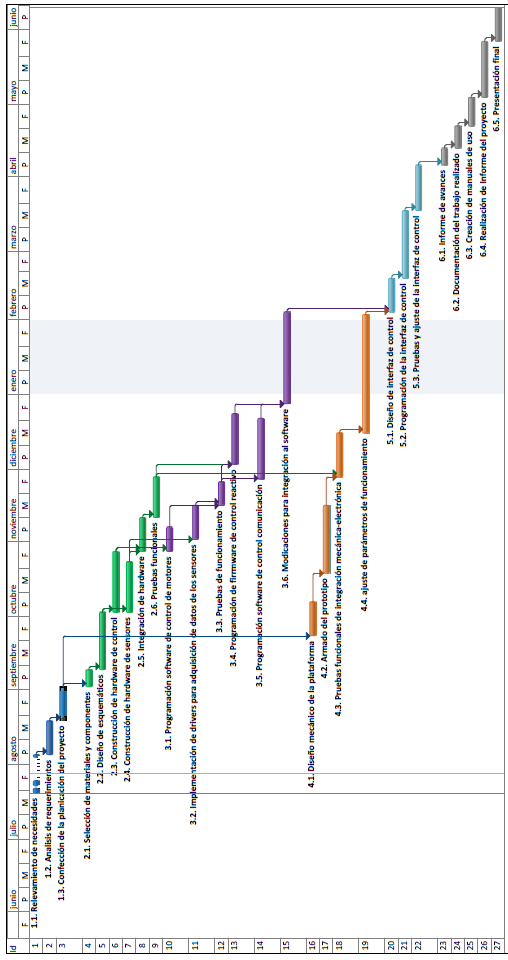
\includegraphics[width=\textwidth]{./Figures/Gantt.PNG}
%%\caption{Diagrama de Gantt.}
%%\label{fig:gantt2}
%%\end{figure}
%%
%%\pagebreak
%%
%%\subsection{Diagrama de Precedencias}
%%Se confeccionó también un diagrama de Precedencias o de Activity on Node (AON), con la finalidad de resaltar las tareas cuyos retrasos podrían resultar críticos para la concreción del trabajo. En rojo se indica el camino crítico, como puede apreciarse en la figura \ref{fig:AoN}
%%
%%\begin{figure}[htpb]
%%\centering 
%%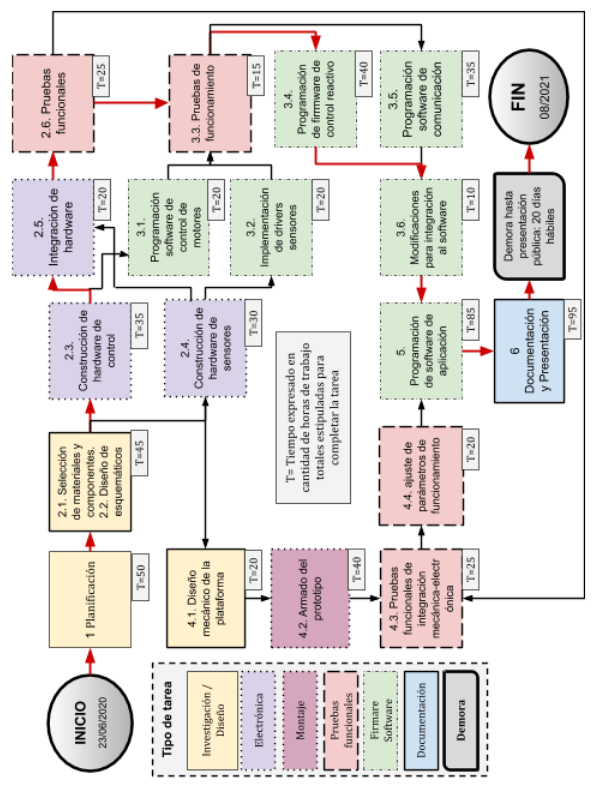
\includegraphics[width=12cm]{./Figures/AoN.png}
%%%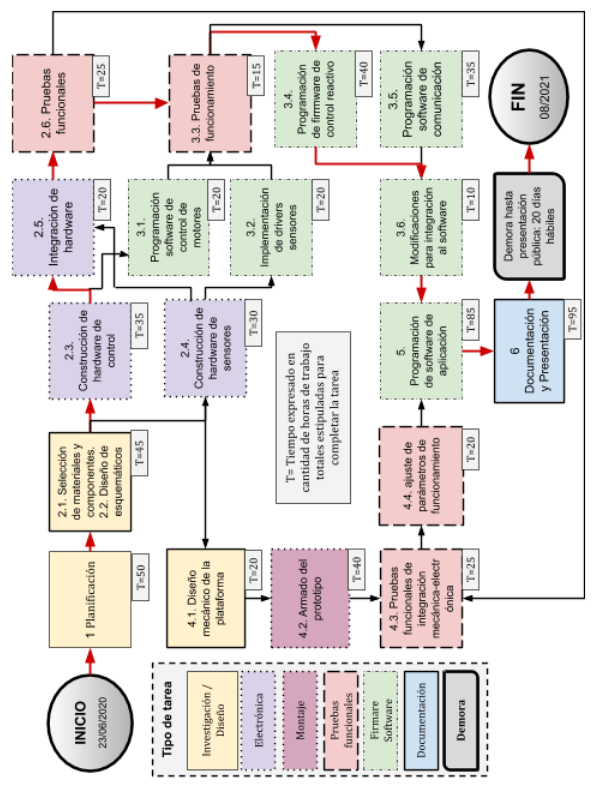
\includegraphics[width=\textwidth]{./Figures/AoN.png}
%%\caption{diagrama de Precedencias o de Activity on Node (AON).}
%%\label{fig:AoN}
%%\end{figure}
%%\pagebreak
%
%\subsubsection{Supuestos iniciales del proyecto}
%
%Para el desarrollo de este trabajo se supuso inicialmente que:
%
%\begin{itemize}
%	\item Se iba a contar con disponibilidad de los laboratorios e instrumental de la  Secretaría de Ciencia, Tecnología e innovación productiva. UTN. Buenos Aires, para cubrir la tarea de desarrollo.
%	\item Se iba a disponer de tiempo durante la jornada laboral para la realización del mismo. 
%	\item Se iba a disponer de todos los componentes y herramientas necesarios.
%\end{itemize}
%
%Estos supuestos, incluidos en la planificación del trabajo, se cumplieron solo en parte, ya que la pandemia por COVID-2019 limitaron el acceso a los laboratorios e instrumental, a la vez que se incrementó el tiempo necesario para las actividades laborales desarrolladas en paralelo al proyecto. 
%
%


 
\chapter{Diseño e implementación} % Main chapter title

\label{Chapter3} % Change X to a consecutive number; for referencing this chapter elsewhere, use \ref{ChapterX}

\definecolor{mygreen}{rgb}{0,0.6,0}
\definecolor{mygray}{rgb}{0.5,0.5,0.5}
\definecolor{mymauve}{rgb}{0.58,0,0.82}

%%%%%%%%%%%%%%%%%%%%%%%%%%%%%%%%%%%%%%%%%%%%%%%%%%%%%%%%%%%%%%%%%%%%%%%%%%%%%
% parámetros para configurar el formato del código en los entornos lstlisting
%%%%%%%%%%%%%%%%%%%%%%%%%%%%%%%%%%%%%%%%%%%%%%%%%%%%%%%%%%%%%%%%%%%%%%%%%%%%%
\lstset{ %
  backgroundcolor=\color{white},   % choose the background color; you must add \usepackage{color} or \usepackage{xcolor}
  basicstyle=\footnotesize,        % the size of the fonts that are used for the code
  breakatwhitespace=false,         % sets if automatic breaks should only happen at whitespace
  breaklines=true,                 % sets automatic line breaking
  captionpos=b,                    % sets the caption-position to bottom
  commentstyle=\color{mygreen},    % comment style
  deletekeywords={...},            % if you want to delete keywords from the given language
  %escapeinside={\%*}{*)},          % if you want to add LaTeX within your code
  %extendedchars=true,              % lets you use non-ASCII characters; for 8-bits encodings only, does not work with UTF-8
  %frame=single,	                % adds a frame around the code
  keepspaces=true,                 % keeps spaces in text, useful for keeping indentation of code (possibly needs columns=flexible)
  keywordstyle=\color{blue},       % keyword style
  language=[ANSI]C,                % the language of the code
  %otherkeywords={*,...},           % if you want to add more keywords to the set
  numbers=left,                    % where to put the line-numbers; possible values are (none, left, right)
  numbersep=5pt,                   % how far the line-numbers are from the code
  numberstyle=\tiny\color{mygray}, % the style that is used for the line-numbers
  rulecolor=\color{black},         % if not set, the frame-color may be changed on line-breaks within not-black text (e.g. comments (green here))
  showspaces=false,                % show spaces everywhere adding particular underscores; it overrides 'showstringspaces'
  showstringspaces=false,          % underline spaces within strings only
  showtabs=false,                  % show tabs within strings adding particular underscores
  stepnumber=1,                    % the step between two line-numbers. If it's 1, each line will be numbered
  stringstyle=\color{mymauve},     % string literal style
  tabsize=2,	                   % sets default tabsize to 2 spaces
  title=\lstname,                  % show the filename of files included with \lstinputlisting; also try caption instead of title
  morecomment=[s]{/*}{*/}
}
En este capítulo se enumeran y desarrollan los aspectos considerados a la hora diseñar el robot. Se tuvieron en cuenta los alcances establecidos como así también las posibilidades económicas de solventar el proyecto.
%----------------------------------------------------------------------------------------
%	SECTION 1
%----------------------------------------------------------------------------------------
\section{Diseño de hardware}

En esta sección se detallan los componentes y módulos electrónicos que forman parte del robot. Se detalla la función que desempeña cada uno de ellos. En la figura \ref{fig:diagramaini} se puede apreciar un diagrama en bloques de los módulos que conforman el robot.


\begin{figure}[h]
	\centering
	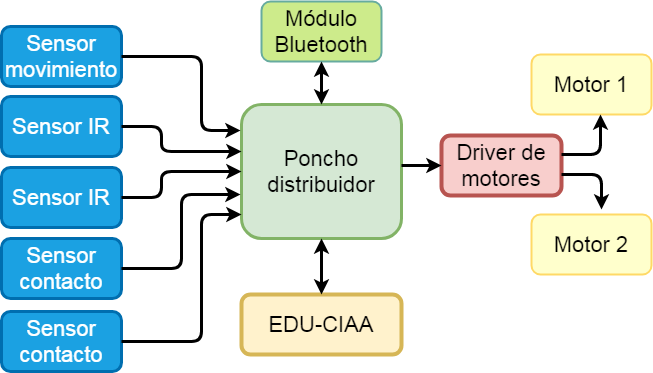
\includegraphics[width=12cm]{./Figures/diagini.PNG}
	\caption{Diagrama en bloques del robot.}
	\label{fig:diagramaini}
\end{figure}



	\subsection{Poncho}
Se denominación  “Poncho”  se utiliza entre la comunidad del proyecto CIAA para referirse a una  placa de expansión de “Shield”  que se conecta sobre algún procesador de la familia CIAA.  Para este proyecto se diseñó un poncho para facilitar las conexiones de la placa EDU-CIAA con los sensores, actuadores y el módulo de comunicación bluetooth.

		\subsubsection{Diseño esquemático del poncho}

El poncho consta de conectores para las señales de entrada:

\begin{itemize}
	\item Sensores infrarrojos (2).
	\item finales de carrera (2).
	\item sensor de movimiento (1).
\end{itemize}

A su vez, permite la conexión con los dispositivos de salida

\begin{itemize}
	\item Módulo de control de motores.
	\item Relé actuador (en la placa).
	\item Buzzer y LEDs (en la placa).
\end{itemize}

La placa posee conexionado para montar un módulo HC-05 de comunicación bluetooth y un conector destinado a dispositivos I2C (como podría ser un módulo de girósocpo o acelerómetro).

		\subsubsection{Diseño PCB del poncho}


La placa fue diseñada durante la cursada de la asignatura “diseño de circuitos s, según los lineamientos expuestos en la documentación para ponchos CIAA. Se procedió a la fabricación de la placa utilizando medios caseros de manufactura.

El diseño de PCB se realizó con el software KiCad \citep{KiCad} (Versión 5.1.9), el cual es un paquete de software para el diseño de circuitos electrónicos o EDA (Electronic Design
Automation). En la figura \ref{fig:poncho3d} se observa el modelo 3D de la placa y sus componentes.


\begin{figure}[h]
	\centering
	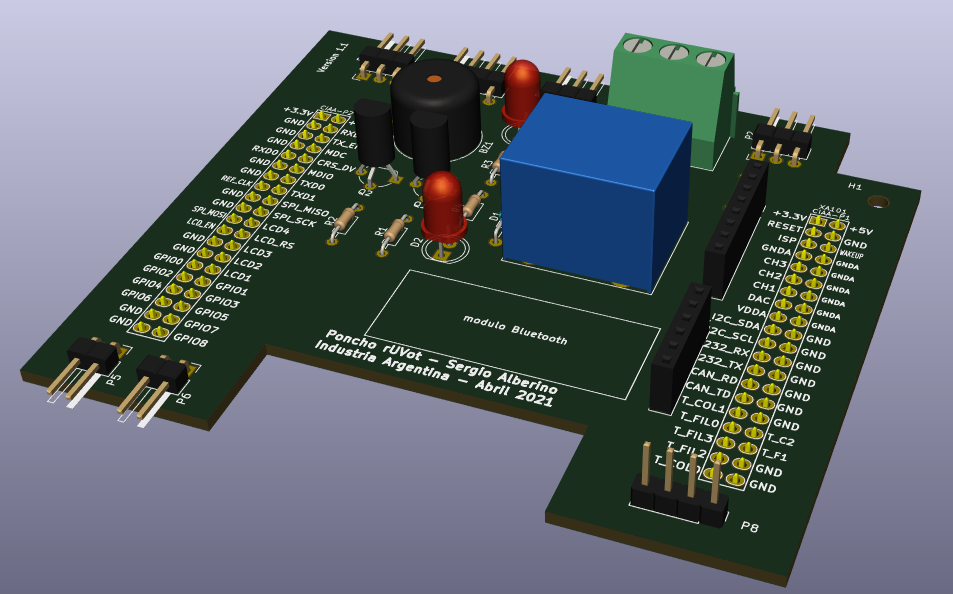
\includegraphics[width=11cm]{./Figures/ponchoiso.PNG}
	\caption{Vista del modelo 3D del poncho rUVot.}
	\label{fig:poncho3d}
\end{figure}


En la figura \ref{fig:esquematico} se presenta el circuito esquemático del poncho donde se puede observar el conexionado eléctrico.

%\begin{figure}[h]
%	\centering
%	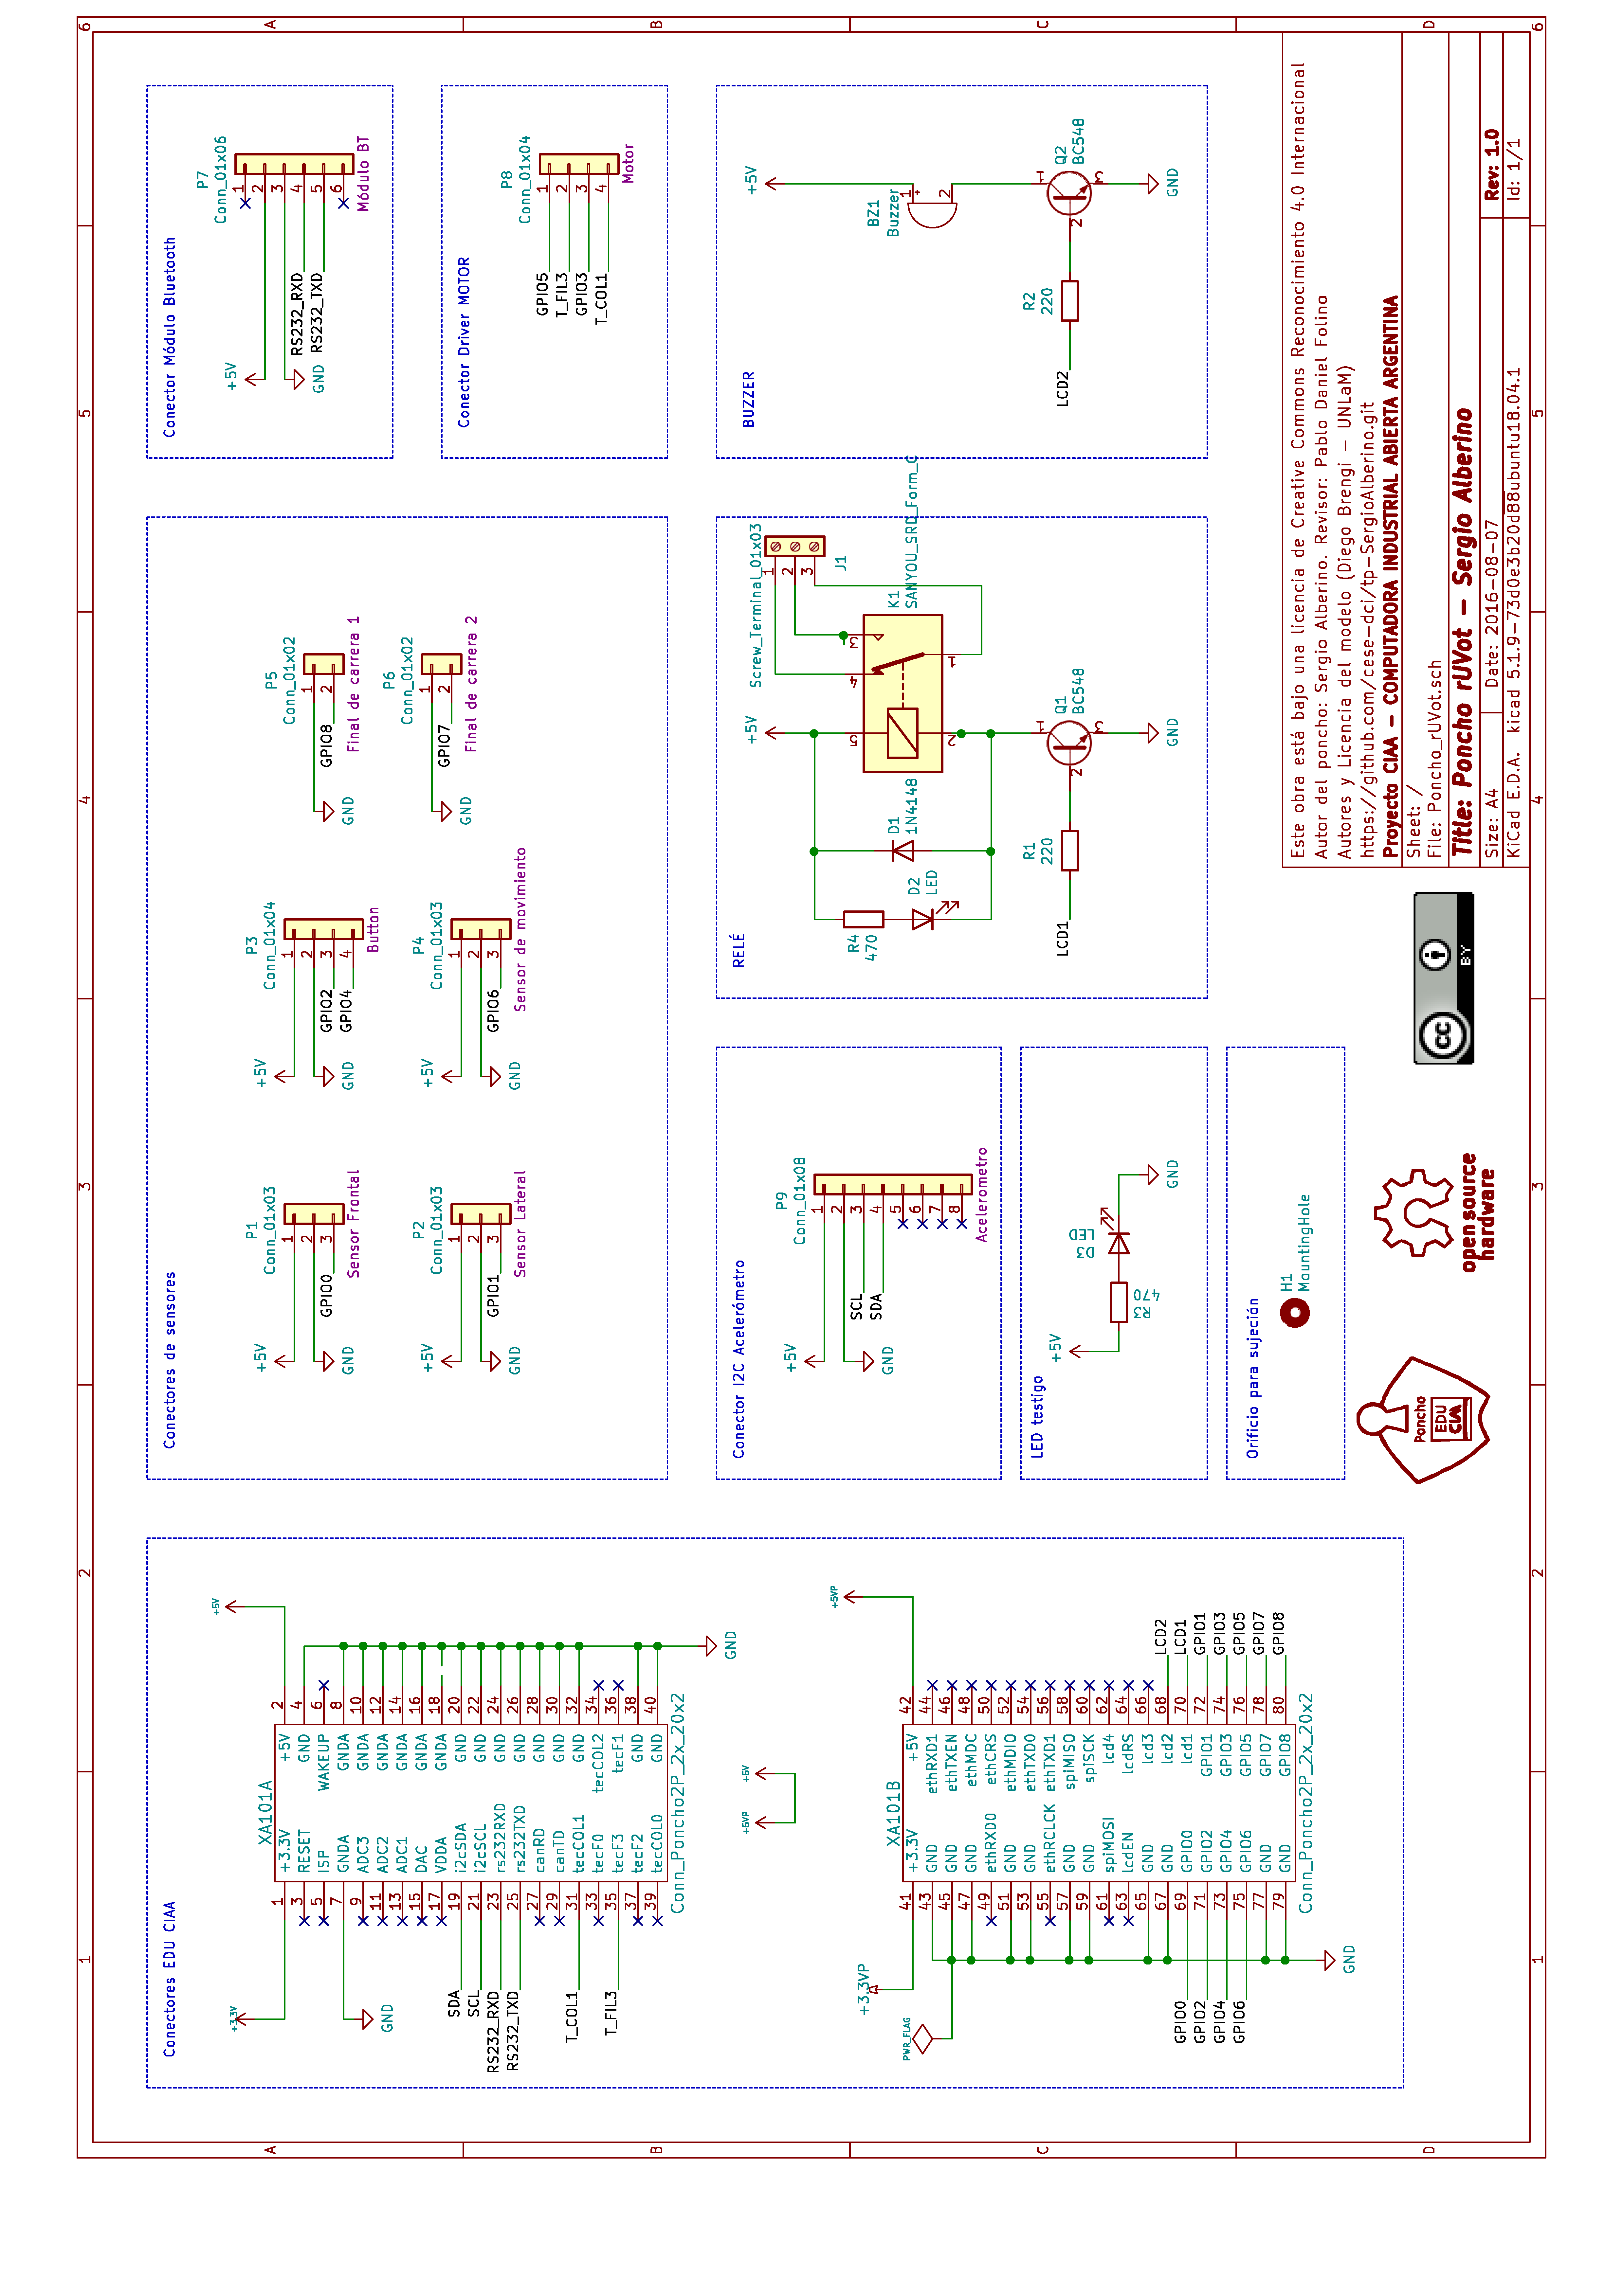
\includegraphics[width=\textwidth]{./Figures/esquematico.png}
%	\caption{Circuito esquemático del poncho.}
%	\label{fig:esquematico}
%\end{figure}
%\pagebreak

\subsection{Esquema de  de comunicaciones}

\section{Diseño mecánico}
\subsection{Gabinete del robot}
\subsection{Motores}

\section{Diseño de software}
\subsection{Tarea de control de motores}
\subsection{Tarea de comunicaciones}







%
%
%
%
%\begin{verbatim}
%\begin{lstlisting}[caption= "un epígrafe descriptivo"]
%	las líneas de código irían aquí...
%\end{lstlisting}
%\end{verbatim}
%
%A modo de ejemplo:
%
%\begin{lstlisting}[label=cod:vControl,caption=Pseudocódigo del lazo principal de control.]  % Start your code-block
%
%#define MAX_SENSOR_NUMBER 3
%#define MAX_ALARM_NUMBER  6
%#define MAX_ACTUATOR_NUMBER 6
%
%uint32_t sensorValue[MAX_SENSOR_NUMBER];		
%FunctionalState alarmControl[MAX_ALARM_NUMBER];	//ENABLE or DISABLE
%state_t alarmState[MAX_ALARM_NUMBER];						//ON or OFF
%state_t actuatorState[MAX_ACTUATOR_NUMBER];			//ON or OFF
%
%void vControl() {
%
%	initGlobalVariables();
%	
%	period = 500 ms;
%		
%	while(1) {
%
%		ticks = xTaskGetTickCount();
%		
%		updateSensors();
%		
%		updateAlarms();
%		
%		controlActuators();
%		
%		vTaskDelayUntil(&ticks, period);
%	}
%}
%\end{lstlisting}




% Chapter Template

\chapter{Ensayos y resultados} % Main chapter title

\label{Chapter4} % Change X to a consecutive number; for referencing this chapter elsewhere, use \ref{ChapterX}

%----------------------------------------------------------------------------------------
%	SECTION 1
%----------------------------------------------------------------------------------------

\section{Pruebas funcionales del hardware}
\label{sec:pruebasHW}

En este capítulo se detallan los ensayos realizados para comprobar el correcto funcionamiento de hardware y firmware, y la interacción de los módulos que componen el robot.

\subsection{Validación de movimientos del robot}
Se verificó que el robot responde a los “estímulos” detectados por los sensores según lo determinado en la librería mde.h, como tabla de configuración de la máquina de estados principal. Se utilizaron los LEDs de la placa EDU-CIAA como testigo del estado tomado por la FSM en cada momento. 

\subsection{Validación módulo de comunicaciones Bluetooth}
\subsection{Validación detección de obstáculos}
\subsection{Validación de navegación autónoma}


\section{Pruebas no Funcionales}
%\subsection{Tarea de comunicaciones} 
% Chapter Template

\chapter{Conclusiones} % Main chapter title

\label{Chapter5} % Change X to a consecutive number; for referencing this chapter elsewhere, use \ref{ChapterX}


%----------------------------------------------------------------------------------------

%----------------------------------------------------------------------------------------
%	SECTION 1
%----------------------------------------------------------------------------------------


En este capítulo se presenta un breve resumen del trabajo realizado, los problemas encontrados y los resultados obtenidos. También se mencionan mejoras a realizar a futuro.

\section{Resultados obtenidos}

El trabajo finalizó con el desarrollo exitoso de un prototipo de robot móvil para tareas de desinfección por efecto de rayos ultravioletas germicidas, donde se cumplieron los requerimientos planteados en la planificación del trabajo.
Se desarrolló con éxito un circuito impreso como placa de expansión de hardware, y un firmware funcional para la placa EDU-CIAA. Asimismo, se verificó el funcionamiento de los modos autónomos y de teleoperación del robot y, por otro lado, se validó que el dispositivo pueda ser utilizado para desinfección sin residuos químicos en espacios públicos y en el hogar.

La planificación, se cumplió dentro de los plazos esperados, aunque se manifestó el riesgo “Imposibilidad de cumplir con los plazos planteados para el desarrollo del proyecto”. Esto se debió a la reducción de tiempo disponible para dedicarle al proyecto,  debido a actividades laborales y académicas. Al haber extendido el plazo para la entrega y haber re-planificado actividades se logró mitigar este inconveniente.


%----------------------------------------------------------------------------------------
%	SECTION 2
%----------------------------------------------------------------------------------------
\section{Conocimientos aplicados}

Durante la realización de este trabajo se aplicaron conocimientos adquiridos en el transcurso de la carrera de especialización. 
En particular, fueron importantes los aportes de las siguientes  asignaturas:


\begin{itemize}
	\item Gestión de proyectos para realizar la planificación y generar toda la documentación inicial.
	\item Ingeniería de software para definir los requerimientos básicos y pensar el proyecto desde las necesidades del usuario. También se aplicaron los conocimientos relativos a la implementación de un repositorio GIT para el resguardo y versionado de toda la documentación del proyecto.
	\item Programación de microcontroladores para la implementación del firmware en C del microcontrolador ARM Cortex-M4 de la placa EDU-CIAA. En la asignatura se presentó todo lo referente a la modularización por archivos implementada en este trabajo y el modelo de máquinas de estado finito.
	\item Protocolos de comunicaciones en sistemas embebidos para conocer las posibilidades de comunicación de la placa EDU-CIAA con otros dispositivos, en particular con el módulo Bluetooth. Tambien en esta asignatura se presentó el entorno MIT App Inventor que se utilizó para el desarrollo de la aplicación de control.
	\item Diseño de Circuitos Impresos para el desarrollo de la placa de expansión de hardware (poncho) utilizada en este trabajo, y el aprendizaje de buenas costumbres de diseño de PCB.
			
\end{itemize}

%----------------------------------------------------------------------------------------
%	SECTION 3
%----------------------------------------------------------------------------------------
\section{Próximos pasos}

Como mejoras a futuro se contempla:

\begin{itemize}
	\item Agregar una unidad de medición inercial o IMU (por su sigla en inglés) como ser un acelerómetro o un giróscopo, para tener informa acerca de la velocidad y orientación del robot  en el modo autónomo. De esta manera se podría ampliar la variedad de recorridos posibles y que no dependan únicamente de las características del entorno. 
	\item Al contar con un puerto I2C en la placa, sería posible incorporar un lector de tarjetas de memoria (tipo SD) para almacenar allí la librería con la que se configura la máquina de estados principal. Con este aditamento sería posible definir o ampliar el comportamiento autónomo del robot sin necesidad de modificar su programación. 		
	\item Ya que la placa de expansión de hardware utiliza un relé para conmutar el módulo UVC, podían desarrollarse otros módulos (intercambiables) con su propia alimentación, que utilicen diferentes lámparas germicidas o que ofrezcan otras prestaciones.  

\end{itemize}
 

%----------------------------------------------------------------------------------------
%	CONTENIDO DE LA MEMORIA  - APÉNDICES
%----------------------------------------------------------------------------------------

\appendix % indicativo para indicarle a LaTeX los siguientes "capítulos" son apéndices

% Incluir los apéndices de la memoria como archivos separadas desde la carpeta Appendices
% Descomentar las líneas a medida que se escriben los apéndices

%% Appendix A

\chapter{Placa de expansión de hardware} % Main appendix title

\label{AppendixA} % For referencing this appendix elsewhere, use \ref{AppendixA}

Diagrama esquemático de la placa de expansión de hardware.

\begin{figure}[h]
	\centering
	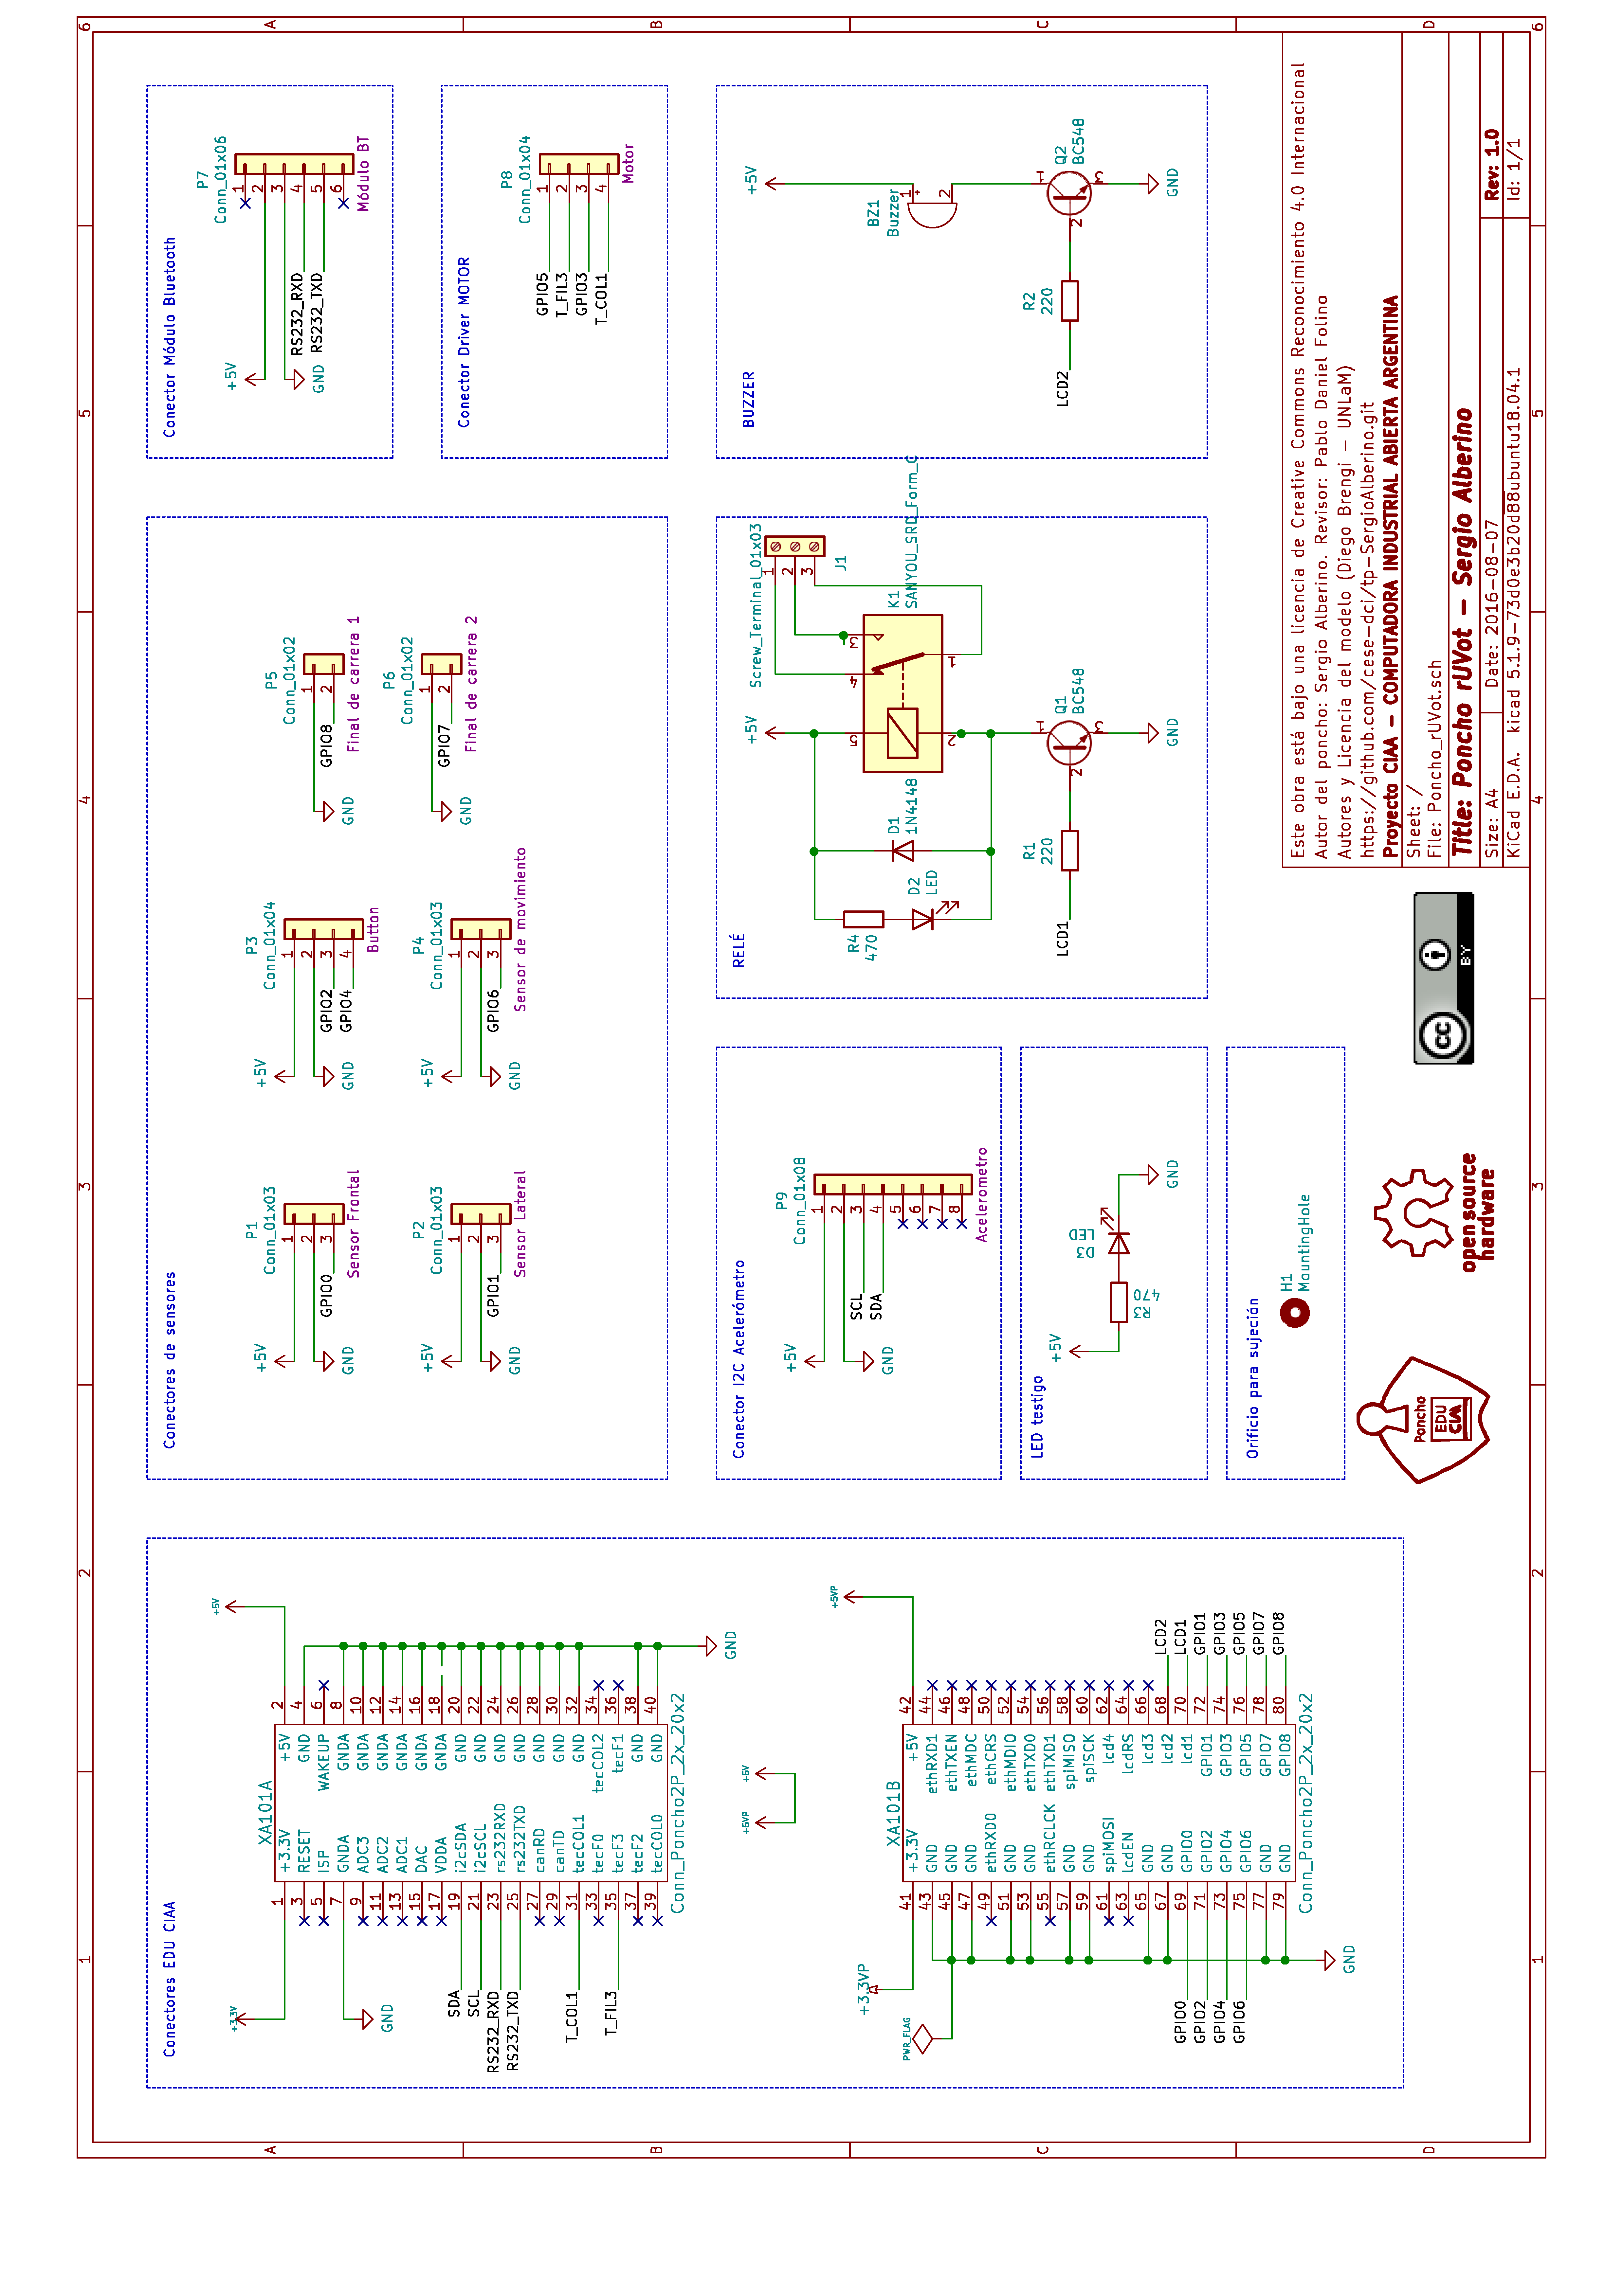
\includegraphics[width=12cm]{./Figures/esquematico.png}
%	\caption{Prototipo armado y cableado, sin la tapa superior.}
%	\label{fig:esquematico}
\end{figure}
%\include{Appendices/AppendixB}
%\include{Appendices/AppendixC}

%----------------------------------------------------------------------------------------
%	BIBLIOGRAPHY
%----------------------------------------------------------------------------------------

\Urlmuskip=0mu plus 1mu\relax
\raggedright
\printbibliography[heading=bibintoc]


%----------------------------------------------------------------------------------------

\end{document}  
